\documentclass{osa-article}

%% Select the journal you're submitting to
%% oe, boe, ome, osac, osajournal
\journal{oe}
% Key:
% Express journals must have the correct journal selected:
% {oe} Optics Express
% {boe} Biomedical Optics Express
% {ome} Optical Material Express
% {osac} OSAC Continuum
% Other OSA journals may use:
% {osajournal} Applied Optics, Advances in Optics and Photonics, Journal of the Optical Society of America A/B, Optics Letters, Optica, Photonics Research

% Uncomment if submitting to Photonics Research.
% ONLY APPLICABLE FOR \journal{osajournal}
% \setprjcopyright

% Set the article type
\articletype{Research Article}
% Note that article type is not required for Express journals (OE, BOE, OME and OSAC)

\usepackage{mathrsfs}
\usepackage{siunitx}
\usepackage{booktabs}
\usepackage{subcaption}

\begin{document}

\title{Non-destructive coherence measurements with double pinholes at FLASH2}

\author{Thomas Wodzinski\authormark{1,2,*}, Mabel Ruiz-Lopez\authormark{2}, Masoud Mehrjoo\authormark{2}, Barbara Keitel\authormark{2}, Marion Kuhlmann\authormark{2}, Maciej Brachmanski\authormark{2}, Swen K\"{u}nzel\authormark{1}, Marta Fajardo\authormark{1}, and Elke Pl\"{o}njes-Palm\authormark{2}}

\address{\authormark{1}GoLP/Instituto de Plasmas e Fus\~{a}o Nuclear, Instituto Superior T\'{e}cnico, 1049-001 Lisboa, Portugal\\
\authormark{2}Deutsches Elektronen-Synchrotron DESY, Notkestrasse 85, 22607 Hamburg, Germany}

\email{\authormark{*}thomas.wodzinski@tecnico.ulisboa.pt} %% email address is required

% \homepage{http:...} %% author's URL, if desired

%%%%%%%%%%%%%%%%%%% abstract %%%%%%%%%%%%%%%%
%% [use \begin{abstract*}...\end{abstract*} if exempt from copyright]

\begin{abstract}

Since 2016 FLASH at DESY in Hamburg operates the variable-gap undulator beamline FLASH2 as a user facility. Young's double pinhole measurements were performed at photon beamline FL24 downstream of the Kirkpatrick-Baez focusing optics, which were installed in 2017. FLASH2 was characterized at wavelengths of 8, 13.5 and 18 nm and under different machine settings. The coherence length was determined from the interference pattern of several pinhole pair separations covering the width of the beam. A blind deconvolution algorithm was implemented to determine the coherence function from the partially coherent interference pattern. Simulations of the patterns including the Kirkpatrick-Baez focusing optics were implemented with WavePropaGator (WPG), a software for X-ray wave front propagation simulations developed at the European XFEL. We present first results of these coherence measurements and simulations.
\end{abstract}


\section{Introduction}

FLASH, the soft X-ray free-electron laser (FEL) in Hamburg, operates since 2016 an additional variable-gap undulator line called FLASH2 \cite{Ploenjes2016}. In contrast to the fixed-gap undulator line FLASH1, the photon energy at FLASH2 can be scanned without changing the electron beam energy.

FLASH generates pulses based on self-amplified stimulated emission (SASE). The stochastic nature of this process can lead to a variation of the beam properties from pulse to pulse. Single-shot photon diagnostics are therefore important to characterize the beam.

Transverse coherence is necessary for experimental techniques like coherent diffractive imaging (CDI) \cite{Chapman2006,WilliamsQuineyPeeleEtAl2007,Abbey2008,Gutt2009,Seibert2011,Zuerch2017, Huang2018, Giewekemeyer2019}, Fourier transform holography (FTH) \cite{Eisebitt2004,Streit-Nierobisch2009,Schaffert2013}, X-ray holographic microscopy (XHM) \cite{Stickler2010,Lider2015}, X-ray ptychography \cite{Rodenburg2007,Bunk2008,RoseSkopintsevDzhigaevEtAl2015,Pfeiffer2017} and X-ray photon correlation spectroscopy (XPCS) \cite{Gruebel2007,Gutt2008, Hruszkewycz2012, Roseker2018, Zhang2018}.

This paper is structured as followed: ...



\section{Basic equations of optical coherence}

In a coordinate system $\vec{r} = (x,y,z) $ a beam with a scalar electric field $ E(\vec{r}, t) $ propagates longitudinally along the $ z $-axis. The transverse coordinates are $ (x,y) $ and $ t $ is the arrival time of the signal at a particular location $ z $.

The mutual coherence function (MCF) \cite{Huang:2013nka} between two points $ r_1 $ and $ r_2 $ is
	\begin{equation}\label{eq:mcf_1}
	\Gamma(\vec{r}_1,\vec{r}_2,t_1,t_2) = \left\langle E(\vec{r}_1, t_1), E^*(\vec{r}_2, t_2) \right\rangle_T
	\end{equation} 
with $ \left\langle \right\rangle_T $ denoting the ensemble average over many radiation pulses over a time interval $ T $ and $ ^* $ the complex-conjugate.

The radiation intensity is $ I(\vec{r},t) = \Gamma(\vec{r},\vec{r},t,t) $.

The complex degree of (mutual) coherence (CDC) $ \gamma $ is defined as the normalized mutual coherence function \cite[eq.4]{BagschikFroemterMuellerEtAl2016a}:
	\begin{equation}\label{eq:cdc}
	\gamma(\vec{r}_1,\vec{r}_2,t_1,t_2) = \frac{\Gamma(\vec{r}_1,\vec{r}_2,t_1,t_2)}{\sqrt{ I(\vec{r}_1,t_1) } \sqrt{I(\vec{r}_2,t_2)}} 
	\end{equation}

where $ \gamma(\vec{r}_1,\vec{r}_2,0) $ describes transverse or spatial coherence, while $ \gamma(0,0,\tau) $ describes longitudinal or temporal coherence.

The spatial or transverse coherence length $ \xi $ is defined as the root mean square (rms) width of the modulus of the CDC \cite[eq.5]{BagschikFroemterMuellerEtAl2016a} along the distance $d$ between two points:

\begin{equation}
    |\gamma_{12}^{\textup{eff}}(d)| \propto \exp{\left[-\frac{d^2}{2 \xi_\textup{x}^2}\right]}
    \label{eq:coherencelength}
\end{equation}

It can be helpful to rather use the term coherence area \cite[fig. 11.2]{Svelto2010} to avoid confusion with the coherence length $L_c$ calculated from the temporal coherence time.

% \begin{figure}[htbp]
%     \centering
%     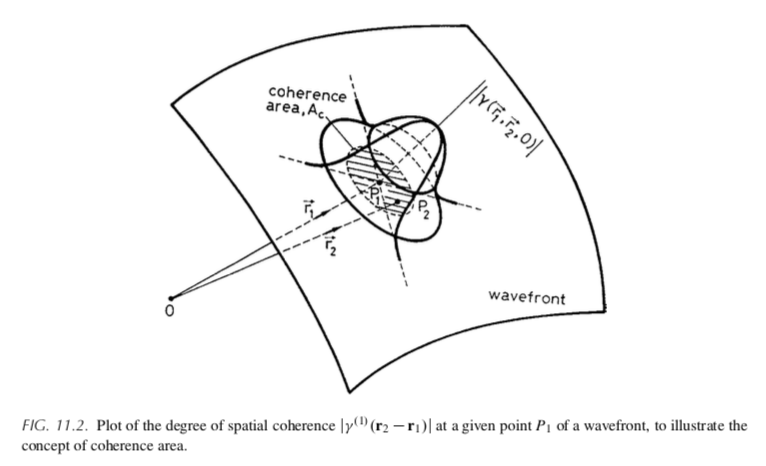
\includegraphics[width=0.7\textwidth]{gfx/Svelto2010fig11p2.png}
%     \caption{Concept of coherence area (from \cite{Svelto2010}).}
%     \label{fig:Svelto2010fig11p2}
% \end{figure}

The size of the beam can be described by its rms width $\sigma_x$:

\begin{equation}
    I(x) \propto \exp\!\left[-\frac{x^2}{2\sigma_x^2}\right]
    \label{eq:beam_rms_width}
\end{equation}

A measure of the degree of coherence is the ratio $ q_x $ between the coherence length $\xi_x$ and the rms width of the beam $\sigma_x $ \cite{MandelWolf1995-Opticalcoherencequantum}:

\begin{equation}
    q_x = \frac{\xi_x}{\sigma_x}
\end{equation}


% \section{Propagation}

% plane at $ z_0 $: $ \vec{s}=(s_x,s_y) $
% plane at $ z_1 $: $ \vec{u}=(u_x,u_y) $

% Huygens-Fresnel principle:

% \begin{equation}
%     E(\vec{u},z_1;\omega) = \int \mathop{d\vec{s}} P_z(\vec{u},\vec{s};\omega) E(\vec{s},z_0;\omega) 
% \end{equation}

% Propagator:
% \begin{equation}
%     P_z(\vec{u},\vec{s};\omega) = \frac{k}{2 \pi i} \frac{e^{ikr}}{r} \chi(\theta)
% \end{equation}

% small angles $ \theta $:

% expand into Taylor: $ kr \approx kz \left( 1 + \frac{|\vec{u}-\vec{s}|^2}{2z^2} - \frac{|\vec{u}-\vec{s}|^4}{8z^4} + ... \right)$

% Fresnel-propagator:

% \begin{align}
%     P_z(\vec{u},\vec{s};\omega) &= \frac{k}{2 \pi i} \frac{e^{ikz}}{z} \exp \left( ik \frac{|\vec{u}-\vec{s}|^2}{2z} \right) \\
%     &= \frac{k}{2 \pi i} \frac{e^{ikz}}{z} \exp \left( ik \frac{|\vec{u}|^2 + |\vec{s}|^2 - 2 \, \vec{u} \cdot \vec{s} }{2z} \right)
% \end{align}

% with $ r \approx z $



\section{Young's double pinhole experiment of a beam with a flat wave front}

The intensity profile $ I(\vec{u}) $ of Youngs' double pinhole experiment \cite[fig. 5.12]{Goodman2015-StatisticalOptics2e} can be described by the interference equation \cite[eq. (2.5-4)]{BahaaE.A.Saleh2007-FundamentalsPhotonics}:

\begin{equation}
    I(\vec{u}) = I_1(\vec{u}) + I_2(\vec{u}) + 2 \sqrt{I_1(\vec{u})} \sqrt{I_2(\vec{u})} \cdot | \gamma_{12}(\tau) | \cdot \cos{\left(\delta(\vec{u})+\alpha_{12}(\tau)\right)}
    \label{eq:interference1}
\end{equation}

with the time delay $ \tau $ between the signals from both pinholes on the detector, the intensities $ I_{1,2} $ of propagated fields $ E_{1,2} $ from pinhole 1 and 2, the rapidly changing phase $ \delta(\vec{u}) $ of $ \gamma_{12} $ describing the interference fringe pattern and the slowly changing phase $ \alpha_{12}(\tau) $.

Under paraxial conditions, with tiny pinholes \cite[eq. (5.2-34)]{Goodman2015-StatisticalOptics2e} and with a small path length difference due to the time delay being smaller than the coherence time $\tau < \tau_c$ we find for $ \delta(\vec{u}) $ and $ \alpha_{12}(\tau) $:

\begin{equation}
    \delta(\vec{u}) \approx 2 \pi \frac{\vec{u} \cdot \vec{d}}{\lambda z}
\end{equation}

and

\begin{equation}
    \alpha_{12}(\tau) \approx \alpha_{12}(0)
\end{equation}

Let the intensity $I_i(\vec{u})$ of pinhole $i$ with diameter $D_i$ on the screen $\vec{u}$ be described by a constant factor $I_i$ and a normalized profile $ \hat{I}_{D_i}(\vec{u}) $:

\begin{equation}
    I_i(\vec{u}) = I_i \cdot \hat{I}_{D_i}(\vec{u})
\end{equation}

In the far-field from the pinholes the intensity profiles of both pinholes can be approximated to overlap at the detector:

\begin{equation}
    \hat{I}_{D_1}(\vec{u}) = \hat{I}_{D_2}(\vec{u})
\end{equation}

The intensity profile of a pinhole in the far-field can be described by the Airy function $ A_{D_i}(\vec{u}) $:

\begin{equation}
    \hat{I}_Di(\vec{u}) = \left| A_{Di}(\vec{u}) \right|^2
\end{equation}

% \begin{equation}
%     I(\vec{u}) = (I_1 + I_2) \cdot I_D(\vec{u}) + 2 \sqrt{I_1 \cdot I_2} \cdot I_D(\vec{u}) \cdot | \gamma_{12}(\tau) | \cdot \cos{\left(2 \pi \frac{\vec{u} \cdot \vec{d}}{\lambda z}+\alpha_{12}(0)\right)}
% \end{equation}

With both pinholes having the same diameter $D=D_1=D_2$ equation \ref{eq:interference1} can be written as:

\begin{equation}
    I(\vec{u}) = (I_1 + I_2) \cdot I_D(\vec{u}) \left[ 1 + \left| \gamma_{12}^{\textup{eff}}(\tau) \right| \cdot \cos{\left(2 \pi \frac{\vec{u} \cdot \vec{d}}{\lambda z}+\alpha_{12}(0)\right)} \right]
\end{equation}

with the effective CDC $\gamma_{12}^{\textup{eff}}(\tau)$ defined as:

\begin{equation}
    \gamma_{12}^{\textup{eff}}(\tau) = 2 \frac{\sqrt{I_1 \cdot I_2}}{I_1 + I_2} \cdot \gamma_{12}(\tau)
\end{equation}

Visibility $ \mathcal{V} $ is defined as:

\begin{equation}
    \mathcal{V} = \frac{I_\textup{max}-I_\textup{min}}{I_\textup{max}+I_\textup{min}}
\end{equation}

At the center of the screen, where $ \tau = 0 $, we can approximate:

\begin{equation}
    \gamma_{12}^{\textup{eff}}(\tau) \approx \gamma_{12}^{\textup{eff}}(0)
\end{equation}

We therefore can determine the modulus of the CDC $ \left| \gamma_{12}(0) \right|$ from the central visibility:

\begin{equation}
    \mathcal{V} = 2 \frac{\sqrt{I_1} \sqrt{I_2}}{I_1 + I_2} \left| \gamma_{12}(0) \right| = \left| \gamma_{12}^{\textup{eff}}(0) \right|
\end{equation}

Usually, one would fit $|\gamma_{12}^{\textup{eff}}(0)|$ as a function of the the pinhole separation $d$ with a Gaussian to determine the transverse coherence length $\xi_x$ from the rms width of this fit (see equation \ref{eq:coherencelength}) \cite[fig.4]{SingerSorgenfreiMancusoEtAl2012}.

% \begin{figure}[htbp]
% 	\centering
% 	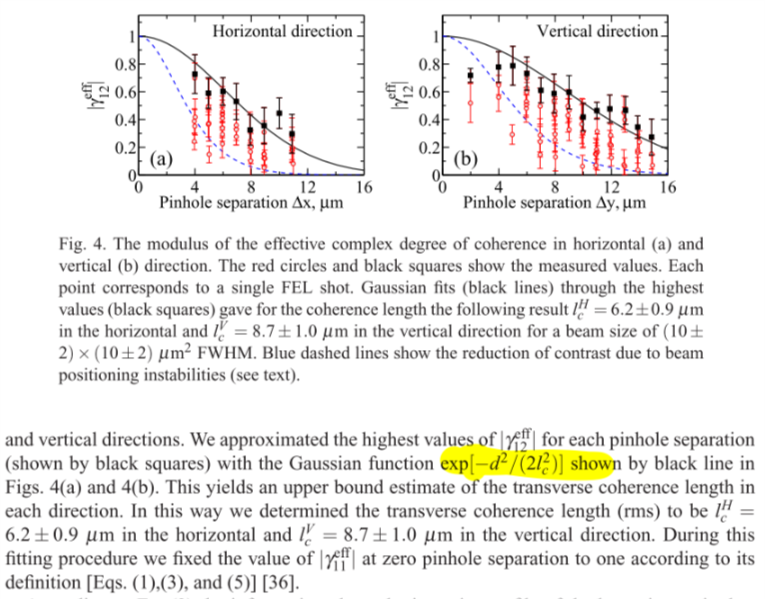
\includegraphics[trim={2cm 10cm 2cm 0cm}, clip, width=0.7\linewidth]{gfx/SingerSorgenfreiMancusoEtAl2012_fig4.png}
% 	\caption{Example of a measurement of the modulus of the complex degree of coherence from the visibility of the central fringes of the interference pattern (from \cite{SingerSorgenfreiMancusoEtAl2012}).}
% 	\label{fig:SingerSorgenfreiMancusoEtAl2012_fig4}
% \end{figure}

These approximations require the wave front to be flat.

\section{Young's double pinhole experiment of a beam with a curved wave front}

If the pinhole pair is not in the focus of the beam the visibility cannot be used as a measure of the CDC. The intensities of each pinhole cannot be assumed to overlap anymore:

\begin{equation}
    \hat{I}_{D_1}(\vec{u}) \neq \hat{I}_{D_2}(\vec{u})
\end{equation}

The focus is located upstream before the pinhole pair at $z_0=0$ in such a way that they are being illuminated by a diverging beam with a curved wave front.

\begin{figure}[h!]
    \centering
    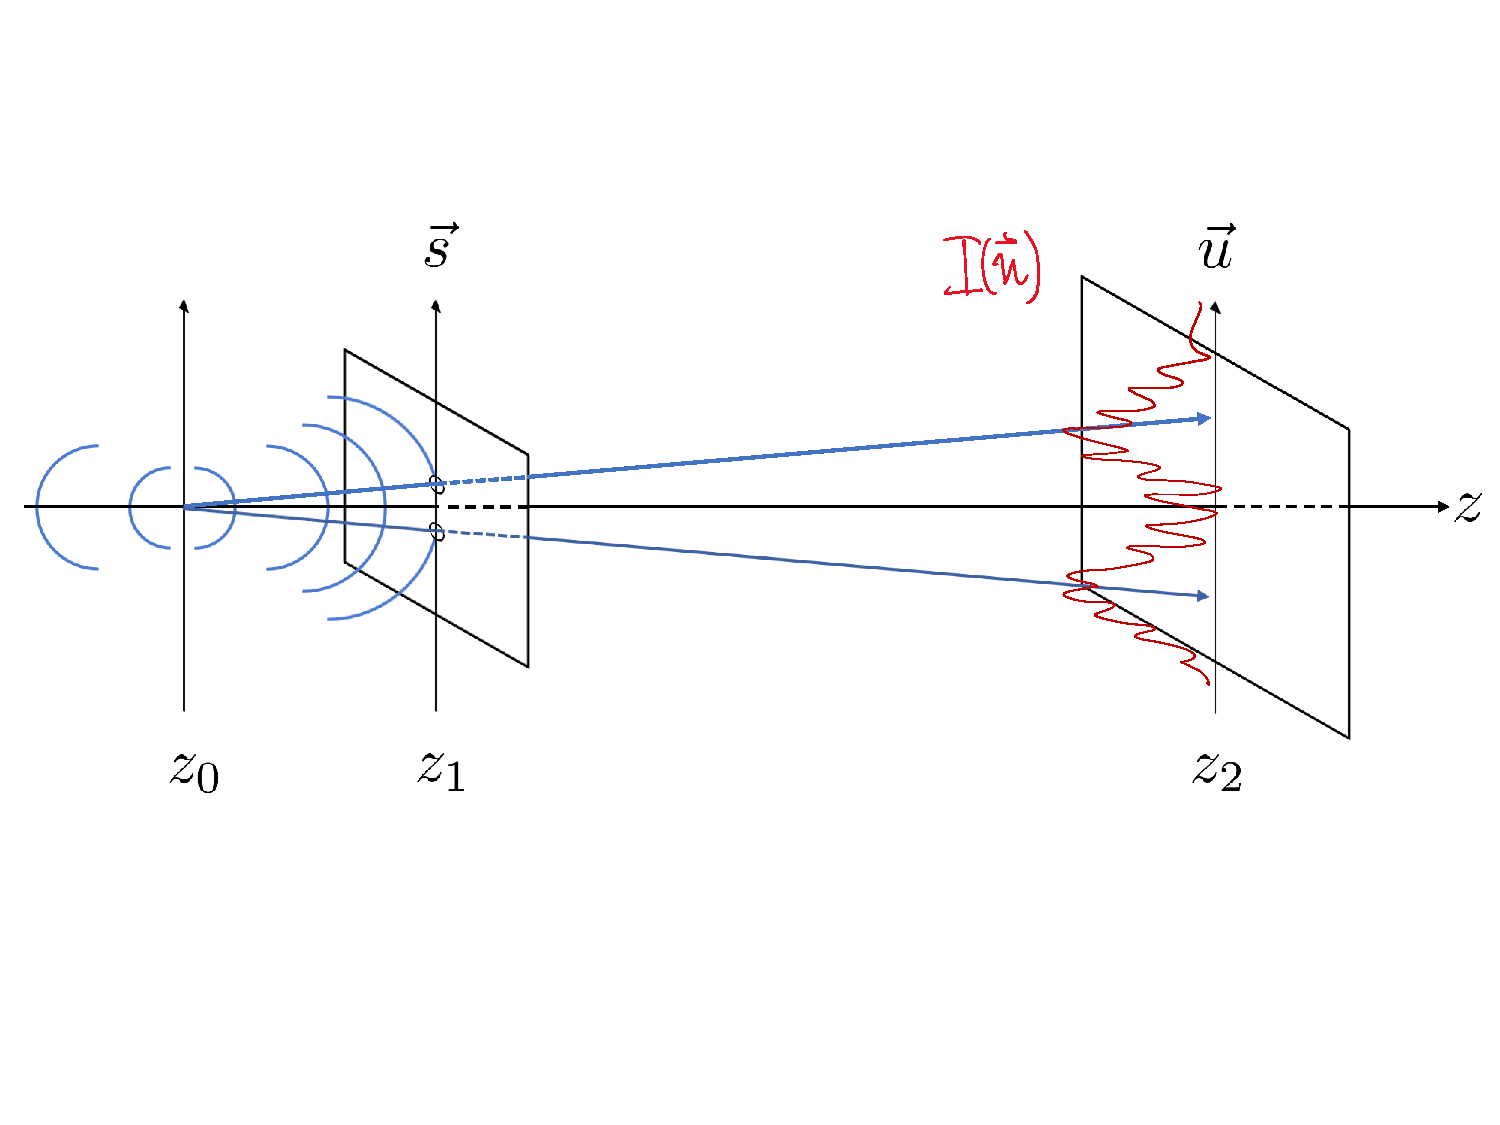
\includegraphics[trim={0cm 0cm 0cm 0cm}, width=0.8\textwidth]{gfx/propagationsketch.pdf}
    \caption{A diverging beam focused at $z_0$ with a curved wave front illuminates a pinhole pair at $z_1$. The resulting interference pattern $I(\vec{u})$ on the screen at $z_2$ samples the curvature.}
    \label{fig:propagationsketch}
\end{figure}

Huygens-Fresnel principle \cite{BornWolfBhatia2002-PrinciplesOptics}:

\begin{equation}
    E(\vec{u},z_2) = \iint P_z(\vec{u},\vec{s}) E(\vec{s},z_1)  \mathop{d\vec{s}}
\end{equation}

with the propagator $P_z$:

\begin{equation}
    P_z(\vec{u},\vec{s}) = \frac{k}{2 \pi i} \frac{e^{ikr}}{r}
\end{equation}



Fresnel-propagator over distance $z$:

\begin{equation}
    P_z(\vec{u},\vec{s}) = \frac{k}{2 \pi i} \frac{e^{ikz}}{z} \exp{\left[ik \frac{\left|\vec{u}\right|^2 + \left|\vec{s}\right|^2 - 2 \vec{u}\cdot\vec{s}}{2z}\right]}
    \label{eq:fresnel-propagator}
\end{equation}

Fraunhofer-propagator over distance $z$:

\begin{equation}
    P_z(\vec{u},\vec{s}) = \frac{k}{2 \pi i} \frac{e^{ikz}}{z} \exp{\left[ik \frac{\left|\vec{u}\right|^2 - 2 \vec{u}\cdot\vec{s}}{2z}\right]}
\end{equation}

Let the wavefront at the pinhole plate be quadratic:

\begin{equation}
    E(\vec{s},z_1) = E_0 \exp{\left[ ik \frac{|\vec{s}|^2}{2z_1} \right]}
    \label{eq:E_at_z1}
\end{equation}

Propagating the field $E(\vec{s},z_1)$ at $z_1$ to $z_2$ over the distance $z = \Delta z_{12} = z_2-z_1$ using Fresnel approximation (eq. \ref{eq:fresnel-propagator}):

\begin{align}
    E(\vec{u},z_2) &= \iint P_z(\vec{u},\vec{s}) E(\vec{s},z_1)  \mathop{d\vec{s}} \\
    &= \iint  \frac{k}{2 \pi i} \frac{e^{ikz}}{z} \exp \left[ ik \frac{|\vec{u}|^2 + |\vec{s}|^2 - 2 \, \vec{u} \cdot \vec{s} }{2z} \right] E(\vec{s},z_1) \mathop{d\vec{s}} \label{eq:E_at_z2_a}
\end{align}

Inserting \ref{eq:E_at_z1} into \ref{eq:E_at_z2_a} leads to the Fresnel scaling theorem for propagating a spherical wave front (\cite["Appendix B", pp.397-400]{Paganin2006}):

% \begin{align}
%     E(\vec{u},z_2) &= \frac{k}{2 \pi i} \frac{e^{ikz}}{z} \exp \left[ ik \frac{|\vec{u}|^2 }{2z}\right] \iint \exp \left[ ik \frac{ |\vec{s}|^2 }{2z} \right] \exp \left[ ik \frac{- 2 \, \vec{u} \cdot \vec{s} }{2z} \right] E(\vec{s},z_1) \mathop{d\vec{s}} \\
%     &= \frac{k}{2 \pi i} \frac{e^{ikz}}{z} \exp \left[ ik \frac{|\vec{u}|^2}{2z} \right]  E_0 \iint  \exp{\left[ ik \frac{|\vec{s}|^2}{2z} \right]}  \exp \left[ ik \frac{ - \vec{u} \cdot \vec{s} }{z} \right] \exp{\left[ ik \frac{|\vec{s}|^2}{2z_1} \right]} \mathop{d\vec{s}} \\
%     &= \frac{k}{2 \pi i} \frac{e^{ikz}}{z} \exp \left[ ik \frac{|\vec{u}|^2}{2z} \right]  E_0 \iint  \underbrace{\exp{\left[ ik \frac{|\vec{s}|^2}{2z_{M}} \right]}}_{\longrightarrow 1 \text{, for Fraunhofer}}  \exp \left[ ik \frac{ - \vec{u} \cdot \vec{s} }{z} \right] \mathop{d\vec{s}} \label{eq:E_at_z2_b}
% \end{align}

\begin{align}
    E(\vec{u},z_2) = \iint  \frac{k}{2 \pi i} \frac{e^{ikz}}{z} \exp{\left[ ik \frac{|\vec{s}|^2}{2z_{M}} \right]} \exp \left[ ik \frac{|\vec{u}|^2 - 2 \, \vec{u} \cdot \vec{s} }{2z} \right] E_0 \mathop{d\vec{s}} \label{eq:E_at_z2_b}
\end{align}

with the scaled distance $z_M$:

\begin{equation}
    z_M = \frac{z_1 \cdot z}{z_1 + z}
\end{equation}

Propagating through one of the two circular pinholes located at $s=+d/2$ away from the optical axis in the plane at $z_1$ with diameter $D$:

\begin{align}
    E(\vec{u},z_2) = \iint_{d/2-D/2}^{d/2+D/2}  \frac{k}{2 \pi i} \frac{e^{ikz}}{z} \underbrace{\exp{\left[ ik \frac{|\vec{s}|^2}{2z_{M}} \right]}}_{\longrightarrow 1 \text{, for Fraunhofer}} \exp \left[ ik \frac{|\vec{u}|^2 - 2 \, \vec{u} \cdot \vec{s} }{2z} \right] E_0 \mathop{d\vec{s}}
\end{align}

If the quadratic term $|\vec{s}|^2 $ in equation \ref{eq:E_at_z2_b} can be neglected we transition from Fresnel to Fraunhofer diffraction \cite[p.46]{BahaaE.A.Saleh2007-FundamentalsPhotonics}, which requires:

\begin{equation}\label{eq:classicaltransition}
	k \frac{\left( d/2 \pm D/2 \right)^2 }{2 z_M} \ll \pi
\end{equation}

With $k=2\pi/\lambda$, the pinhole separation $d$ therefore has to fulfill the following condition:

% When ineq. (\ref{eq:classicaltransition}) is not satisfied, eq. (\ref{eq:fresnel-prop1}) gradually collapses. This gives us a condition for the pinhole separation $ d $ :

\begin{equation}\label{eq:cut-off}
	|d| \ll 2 \sqrt{\lambda z_M} - D
\end{equation}



% In short, relying solely on the Fresnel number, in case of a divergent illumination of the double-pinhole plate, might not be enough assessment for interpreting the intensity observed. Referring to the experimental geometry, $ z_M $ is approximately 0.85 ($ z_p = \SI{6}{m} $ and $ z_0 = \SI{1}{m} $), $ \lambda = \SI{13.5}{nm} $ and $ w = \SI{10}{\micro\meter} $. Thus, $ D_\mathup{cut-off} \approx \SI{20}{\micro\meter} $. It should be noted that $ D $ has been determined for an ideal experiment and it may potentially change with the systematical variations. Considering the wavelength and geometry described in \cite{VartanyantsSingerMancusoEtAl2011} for a Young's double pinhole experiment (with a negligible wavefront curvature) at LCLS, $ D_\mathup{max} $ is found to be $ D_\mathup{max} \approx \SI{60}{\micro\meter} $. As reported, they used a series of pinholes ranging from \SIrange{2}{15}{\micro\meter} which automatically satisfied ineq. (\ref*{eq:classicaltransition}).


\section{Deconvolution-method to recover the fully coherent intensity}

% \begin{figure}[h!]
%     \centering
%     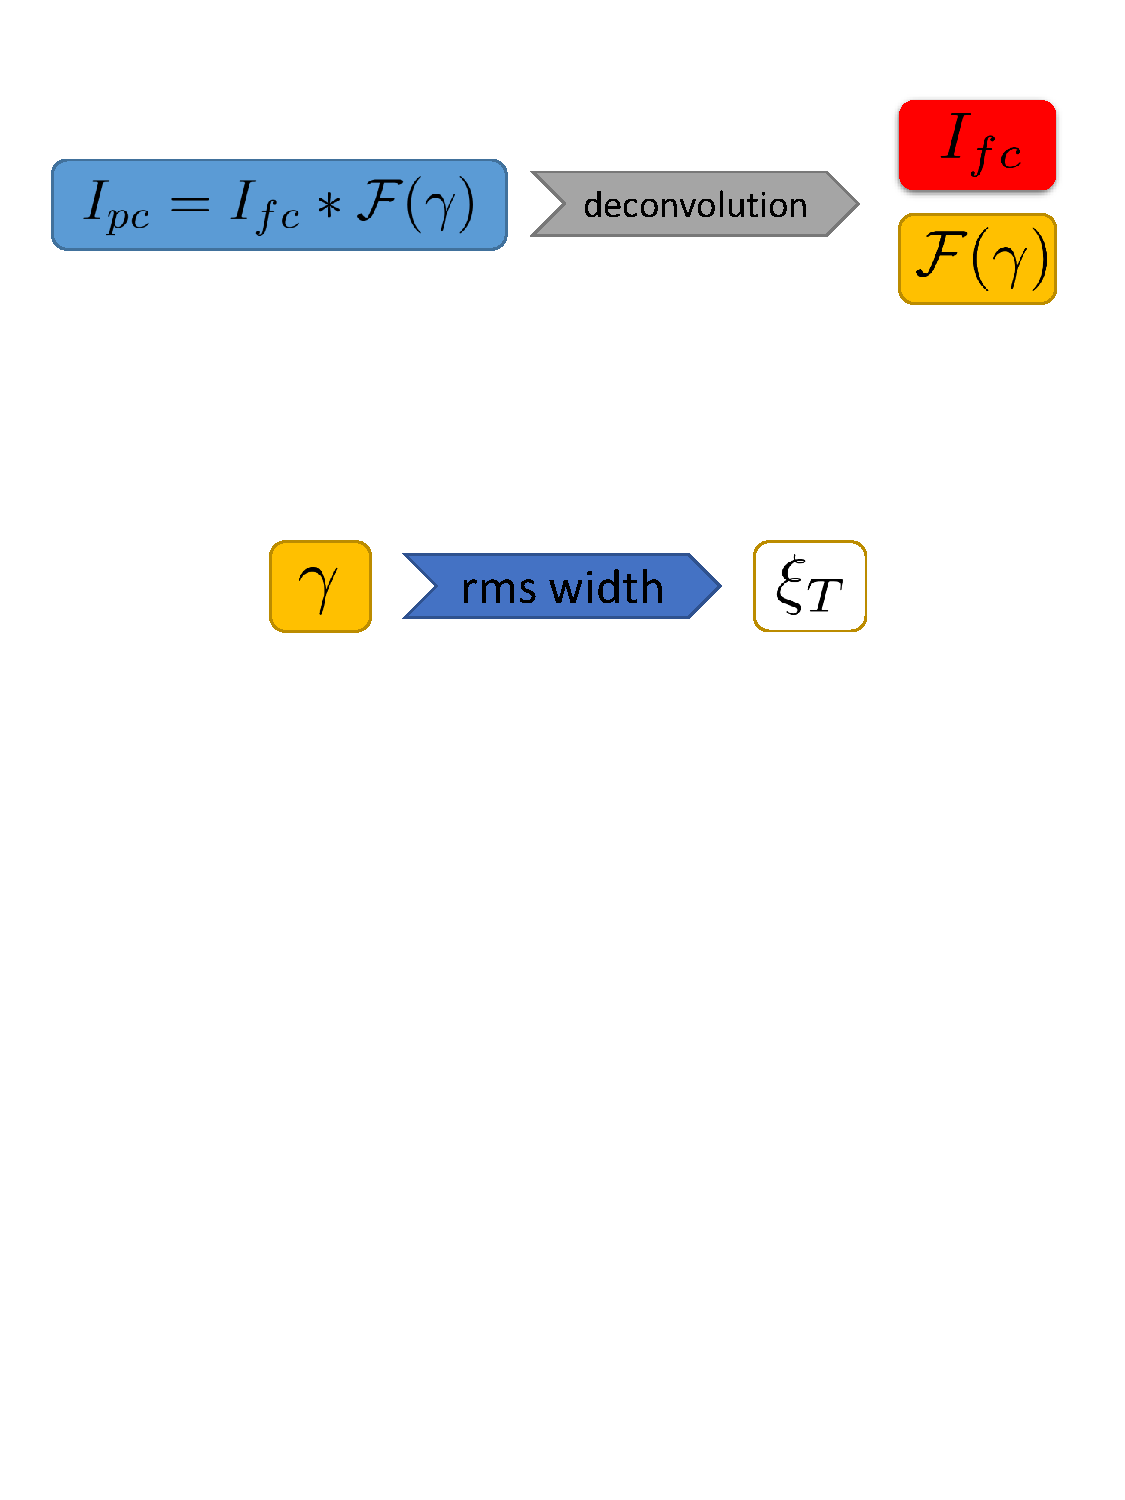
\includegraphics[trim={0cm 15cm 0cm 0cm}, width=0.8\textwidth]{gfx/deconvolution_method_flowchart.pdf}
%     \caption{Deconvolution method to determine the coherence length $\xi$ as the rms width of the modulus of the complex degree of coherence $|\gamma(\vec{r})|$ at the pinhole plate position.}
%     \label{fig:deconvolution_method_flowchart}
% \end{figure}

\begin{figure}[h!]
    \centering
    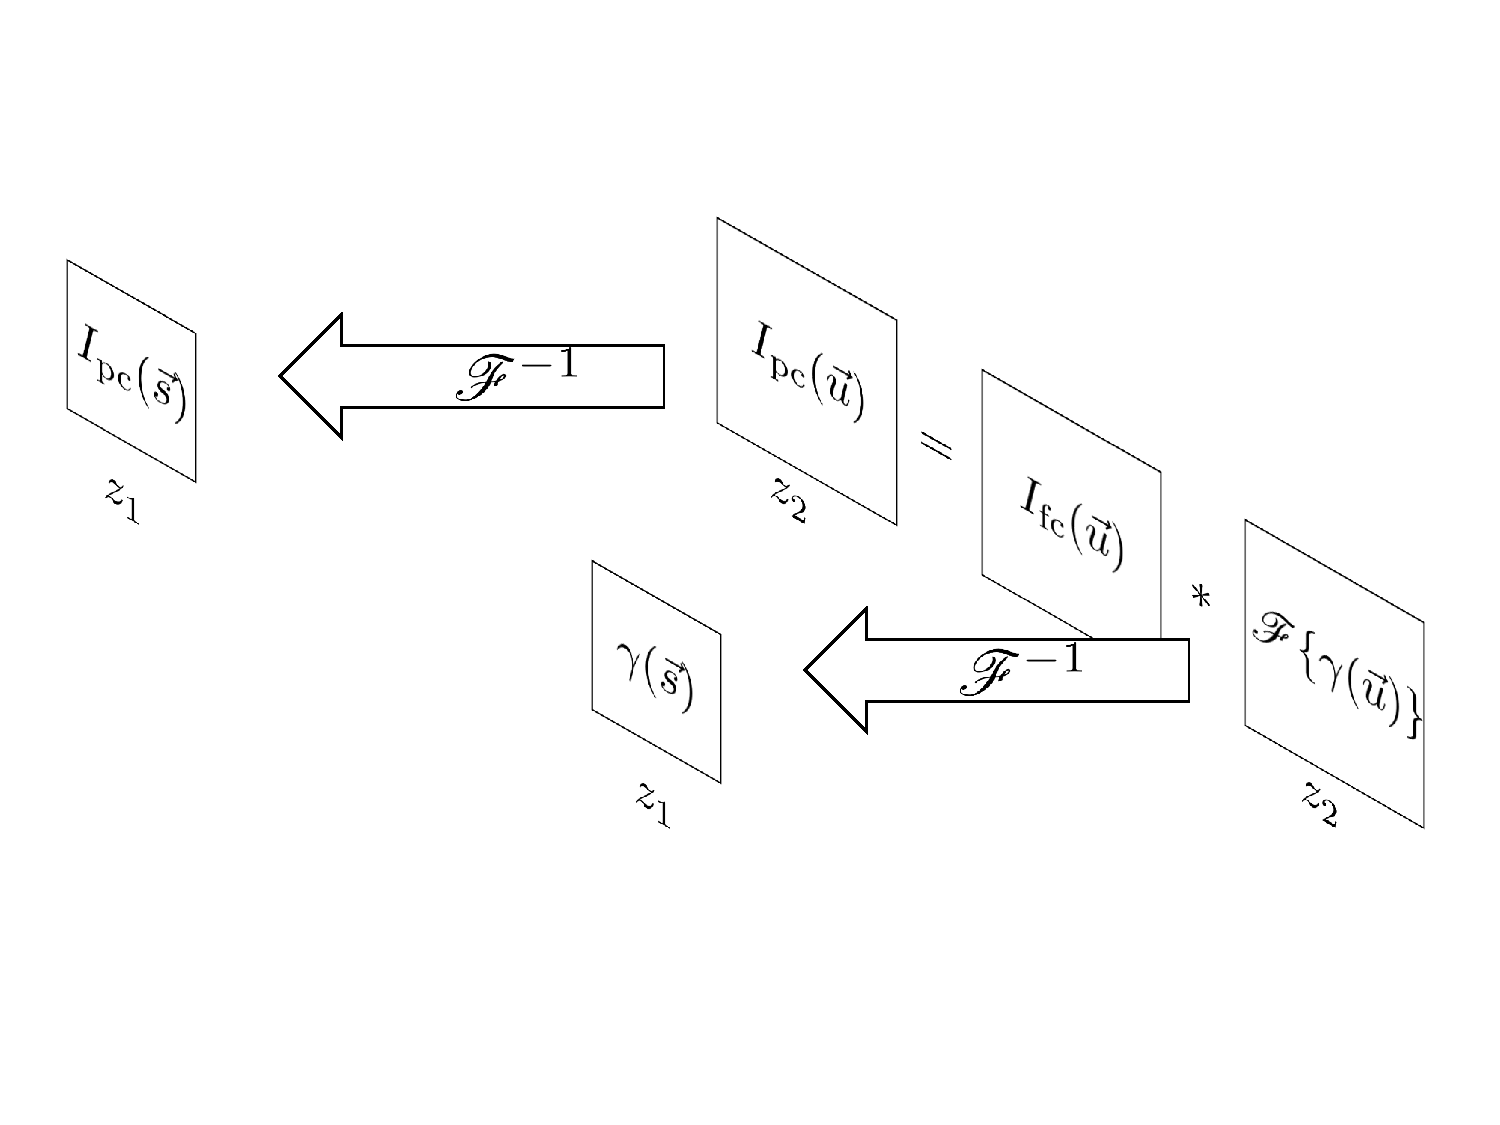
\includegraphics[trim={0cm 0cm 0cm 0cm}, width=0.8\textwidth]{gfx/deconvolution_sketch.pdf}
    \caption{Deconvolution method to determine the coherence length $\xi$ as the rms width of the modulus of the complex degree of coherence $|\gamma(\vec{r})|$ at the pinhole plate position.}
    \label{fig:deconvolution_method_flowchart}
\end{figure}

The measured partically coherent intensity at the detector $I_{\textup{pc}}(\vec{u})$ can be expressed as a convolution of the fully coherent intensity $I_{\textup{fc}}(\vec{u})$ with the Fourier-transformed of the CDC $\mathscr{F}\{\gamma(\vec{u})\}$ \cite[eq.33]{VartanyantsRobinson2001}:

% (see \cite[(eq.33)]{VartanyantsRobinson2001} \cite[(eq.23)]{WilliamsQuineyPeeleEtAl2007} (citing \cite{LinPatersonPeeleEtAl2003} (citing \cite{Nugent1991})), \cite[(eq.1)]{WhiteheadWilliamsQuineyEtAl2009} and \cite[(eq.5)]{ClarkHuangHarderEtAl2012}):

\begin{equation}
    I_{\textup{pc}}(\vec{u}) = I_\textup{fc}(\vec{u}) \ast \mathscr{F}\{\gamma(\vec{u})\}    
\end{equation}

To determine the modulus of the CDC $\gamma(\vec{s})$ at the pinhole plate position $z_1$ we apply the inverse Fourier-transform to back-propagate.

The transverse coherence length $\xi$ is the rms width of  $|\gamma(\vec{s})|$ (see equation \ref{eq:coherencelength}).


\section{Experiment}

Double pinholes with a diameter of \SI{10}{\micro\meter} were illuminated at the beamline FL24 of FLASH2 positioned \SI{1067}{mm} downstream of a focus produced by the Kirkpatrick-Baez focusing optics "KAOS" which is equipped with bendable mirrors. The experiment had different configurations. First, by using a Hartmann-WFS the focus was set to be at the position where a PMMA setup would be placed to create imprints along the caustic. 

After the focus was established the end of the beamline was changed to replace the WFS with a XUV detector, a Princeton Instruments PIXIS XO-1024B with 1024x1024 pixels of $\SI{13}{\micro\meter} \times \SI{13}{\micro\meter}$ size, positioned \SI{5781}{mm} from the position of the pinhole-plate which was itself \SI{1067.5}{mm} downstream of the PMMA focus.

The work on the PMMA imprints was done in collaboration with a group from the Institute of Physics, Academy of Sciences of the Czech Republic from Prague around Jarom\'{i}r Chalupsk\'{y}. They did similar measurements at LCLS \cite{Chalupsky2015PRA}.

After the PMMA imprints were performed the setup was moved out of the beampath and the pinhole plate was inserted. A fluorescent coating on a plate attached to the pinhole plate allowed an additional characterization of the beam size and position with an optical camera. The pinhole plate was movable in the transverse plane, allowing the positioning of several pinhole pairs ranging from \SIrange{107}{1557}{\um} in horizontal and vertical configuration to the beam.

For each pinhole pair consecutive single-shot measurements were recorded over a time of around 5 minutes. The optical beamline cameras recording the fluorescent screen were attached to the data acquisition system (DAQ). Each recorded image had a timestamp. These were later correlated in the data processing with the recorded images of the XUV camera. Background images were recorded with the beam hitting the fluorescent screen between two pinhole pairs.

WFS measurements were done before and after each PMMA measurement, which lasted several hours each.

A second measurement for each pinhole pair was done with the focus changed in such a way, that the beam size at the pinhole position had around half the size than before.

FLASH2 was set to operate at three different wavelengths, \SI{8}{nm}, \SI{13.5}{nm} and \SI{18}{nm}. The machine settings are listed in table \ref{tab:machine_settings}.

\begin{figure}[htbp]
    \centering
    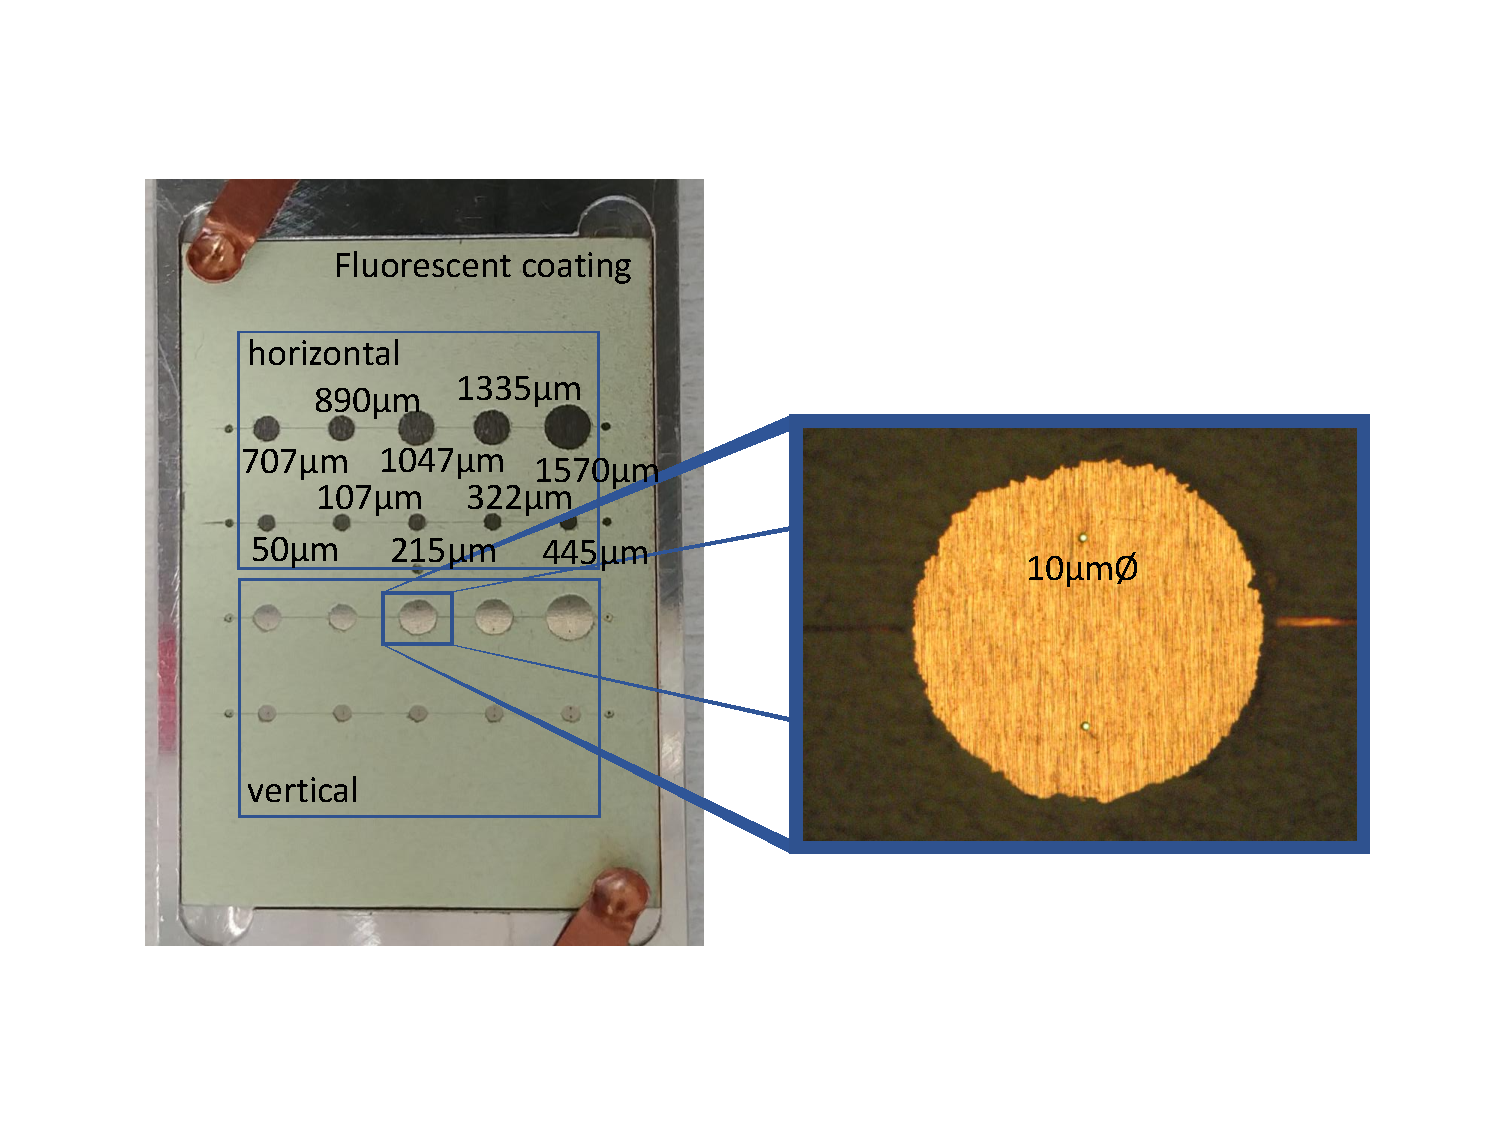
\includegraphics[width=0.8\textwidth]{gfx/pinholeplate_with_microscope_example.pdf}
    \caption{Double pinhole plate with fluorescent coating. An microscope image shows the pinholes with a diameter of \SI{10}{\micro\meter}}
    \label{fig:pinholeplate_with_microscope_example}
\end{figure}

\begin{figure}[htbp]
    \centering
    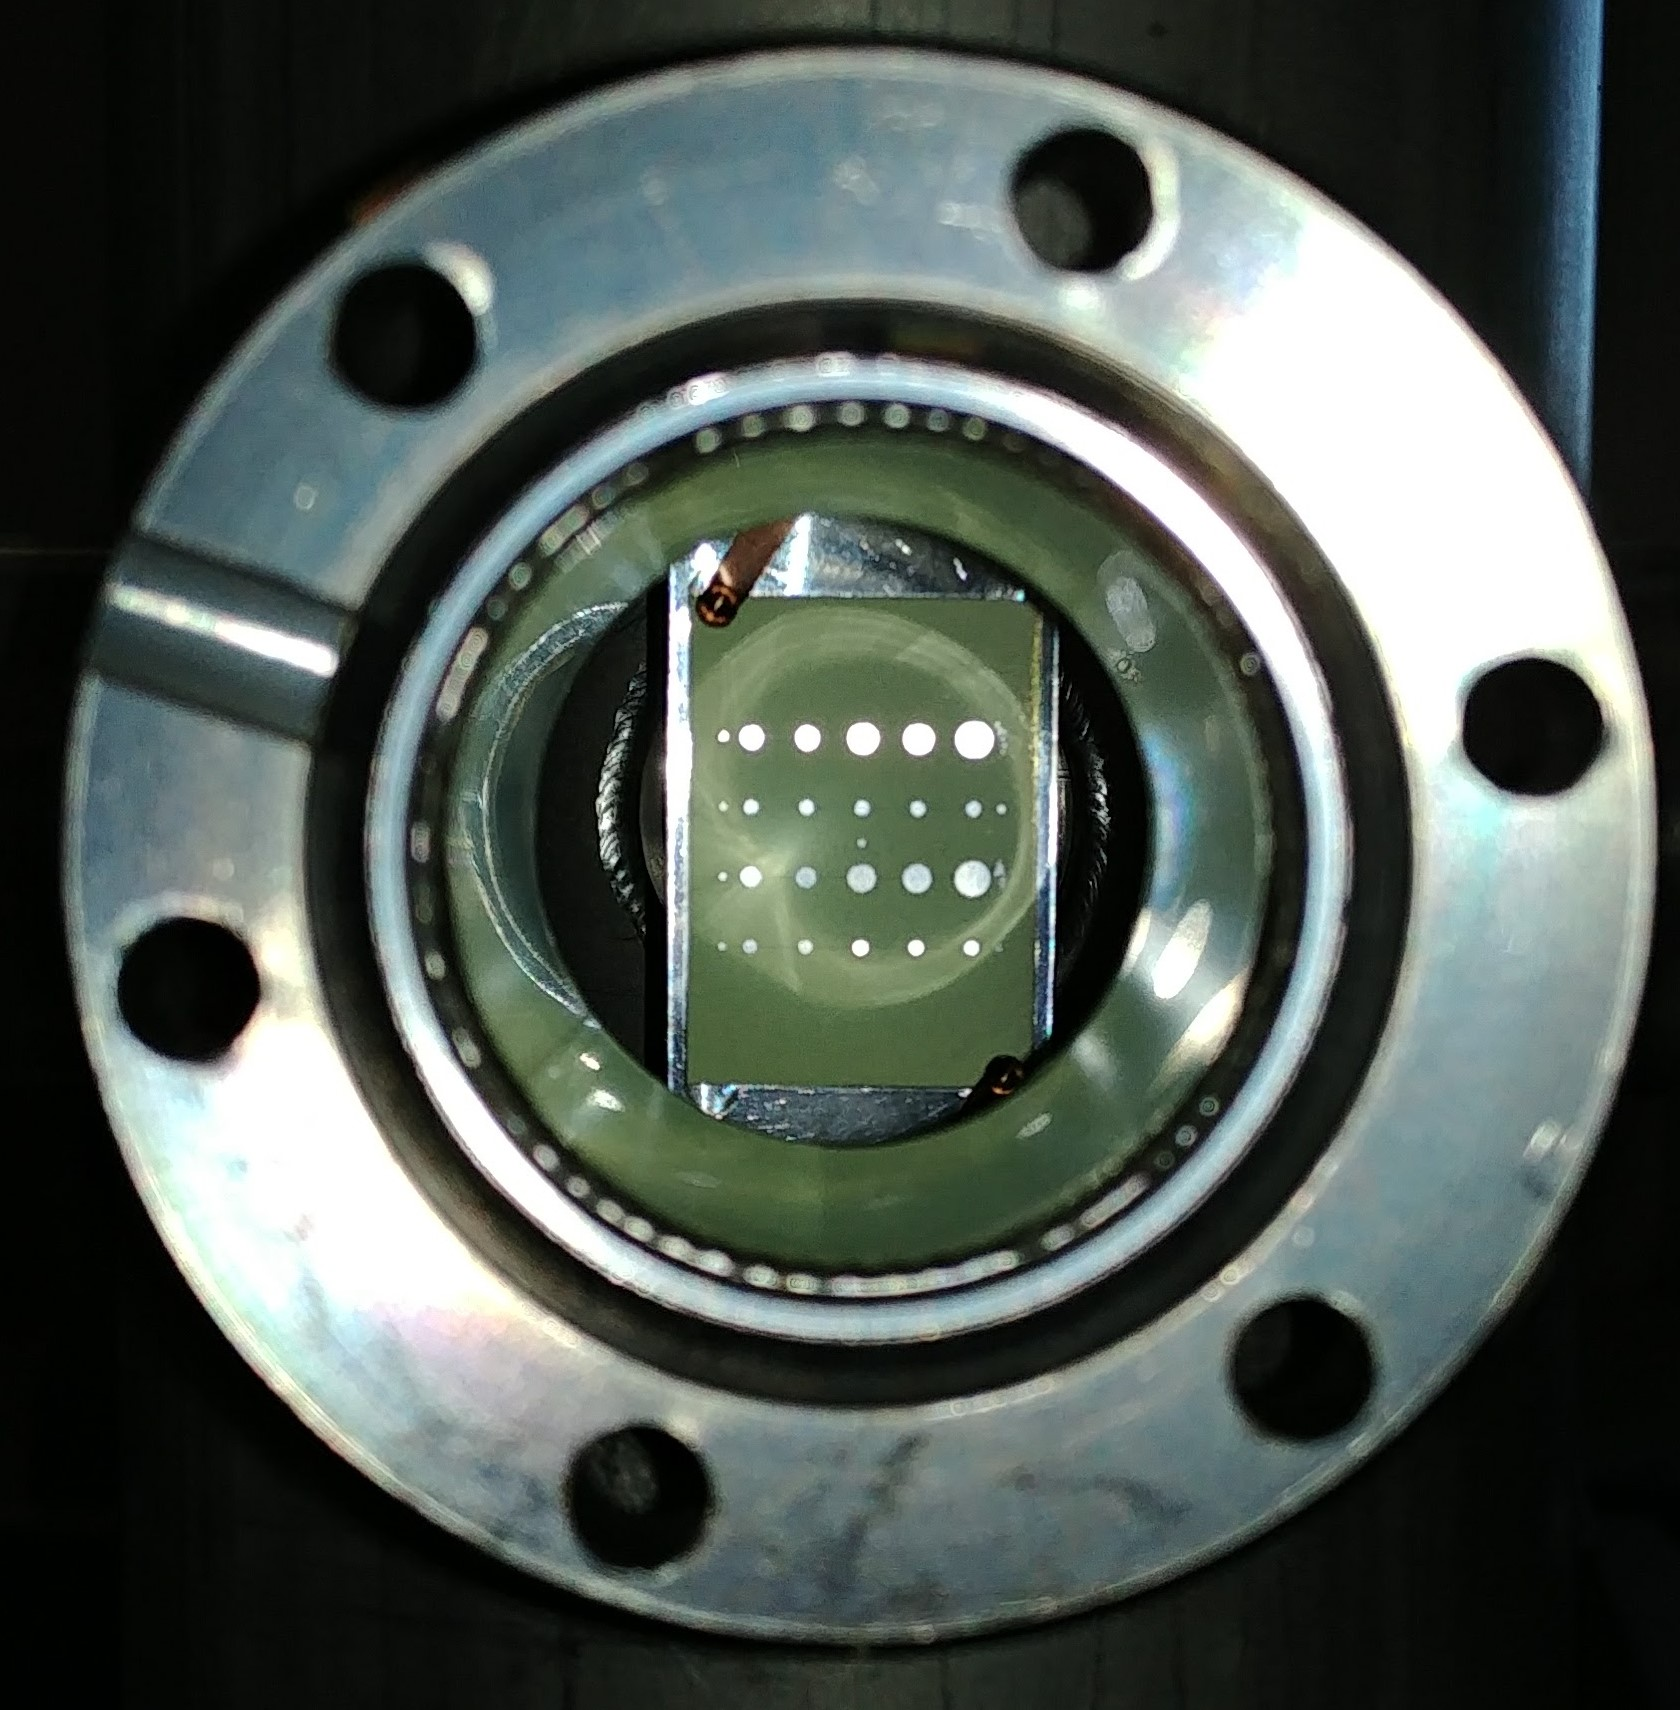
\includegraphics[width=0.5\textwidth]{gfx/pinholeplate_in_chamber.jpg}
    \caption{Double pinhole plate with fluorescent coating mounted inside a movable chamber.}
    \label{fig:pinholeplate_in_chamber}
\end{figure}

\begin{figure}[htbp]
    \centering
    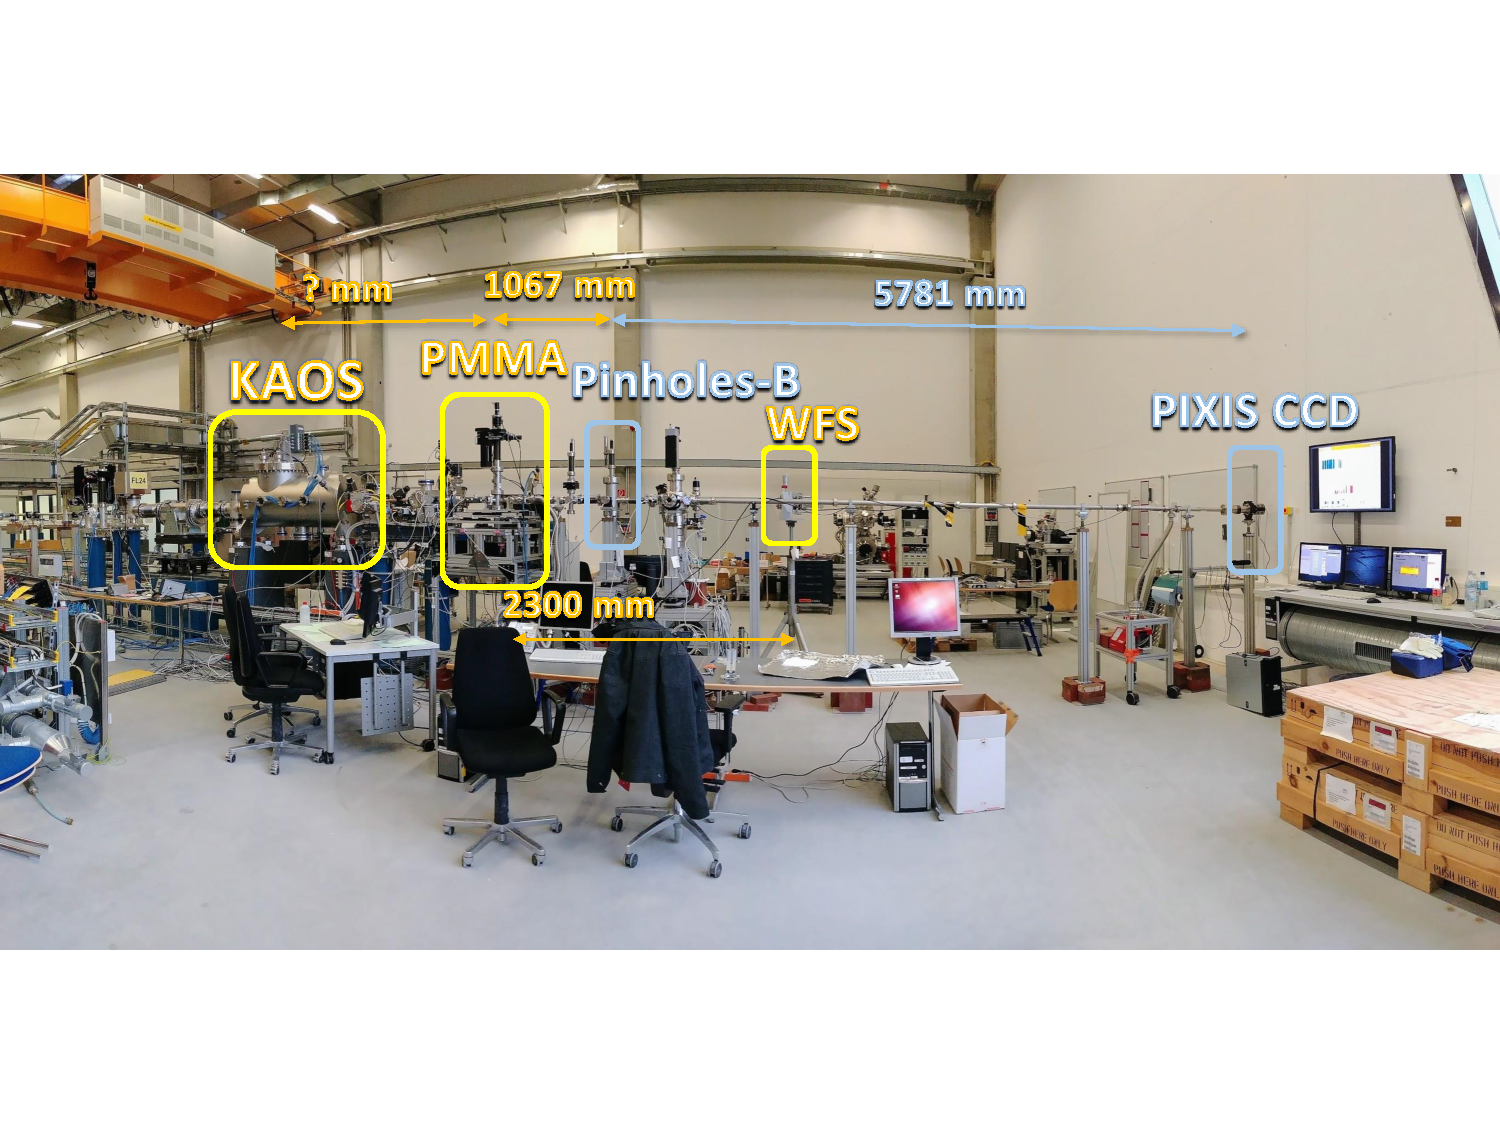
\includegraphics[width=0.8\textwidth]{gfx/setup_sketch_with_photo.pdf}
    \caption{Double pinhole setup at beamline FL24 at FLASH2/DESY}
    \label{fig:DPH_setup}
\end{figure}

\begin{figure}[htbp]
    \centering
    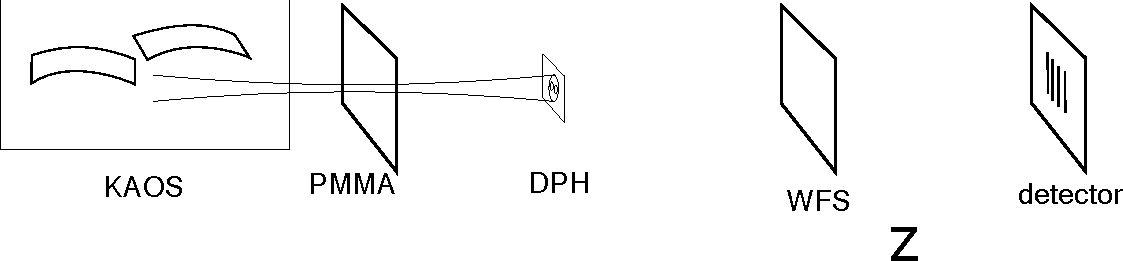
\includegraphics[width=0.8\textwidth]{gfx/sketch_dph_setup.pdf}
    \caption{Double pinhole setup at beamline FL24 at FLASH2/DESY}
    \label{fig:DPH_setup}
\end{figure}

% Please add the following required packages to your document preamble:
% \usepackage{booktabs}
\begin{table}[]
\begin{tabular}{@{}llll@{}}
\toprule
run                  & 26.11.2017             & 27.11.2017           & 29.11.2017                                                                          \\ \midrule
Wavelength           & \SI{18}{nm}                   & \SI{8}{nm}                  & \SI{13.5}{nm}                                                                             \\
\# bunches           & 1                      & 1                    & 1                                                                                   \\
bunch charge         & \SI{0.15}{nC}, \SI{1003}{kHz}      & \SI{0.15}{nC}, \SI{1003}{kHz}    & \SI{0.20}{nC}, \SI{1003}{kHz}                                                                   \\
                     & \SI{1010.59}{MeV}            & \SI{1012.34}{MeV}          & \SI{1046.93}{MeV}                                                                         \\
Energy in the tunnel & \SI{77.4}{\micro\joule}          & \SI{53.7}{\micro\joule}         & \SI{527}{\micro\joule}                                                                        \\
Energy in the hall   & \SI{66.7}{\micro\joule}          & \SI{45.1}{\micro\joule}        & \SI{111}{\micro\joule}                                                                    \\
Undulators           & 7 Undulators (\#8 to \#14)    & 12 Undulators (\#3 to \#14) & 12 undulators (\#3 to \#14)                                                                \\
Tapering             & ?                      & no tapering          & \begin{tabular}[c]{@{}l@{}}quadratic tapering\\  last 6 undulators\end{tabular}     \\
Attenuator           & empty                  & empty                & \begin{tabular}[c]{@{}l@{}}$1.62 \times 10^{-3}$ mbar Xe\\  in attenuator\end{tabular} \\
Filters              & Nb 405 nm or Nb 197 nm & empty                & empty                                                                               \\ \bottomrule
\end{tabular}

\caption{Machine settings of FLASH2 during the measurements}
\label{tab:machine_settings}
\end{table}

\section{Data processing}

Since the beamline cameras were recording the images into the data acquisition system, each recorded shot of the fluorescent screen had a timestamp associated to them. The images of the XUV detector were also captured by the DAQ, but were out of sync. The corresponding timestamp for each XUV image had to be determined by hand. With the correct timestamp known, each shot could be correlated with beam energies and positions provided by diagnostics in the beamline. As can be seen in figure \ref{fig:beam_position_vs_energy} the 

\begin{figure}[htbp]
    \centering
    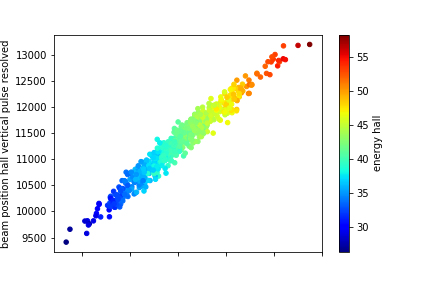
\includegraphics[width=0.5\textwidth]{gfx/beam_position_vs_energy.png}
    \caption{Example of the linear beam position dependence on the beam energy from shot to shot.}
    \label{fig:beam_position_vs_energy}
\end{figure}

The rotation of each image had to be slightly corrected by around $\pm \SI{1}{\degree}$ to align the fringes of the interference pattern vertically. The images of the vertically aligned pinhole pairs were rotated by $\SI{90}{\degree}$.





\section{Beam size at the pinhole plate}

By solving the Fresnel-Kirchoff integral \cite{Floeter2010NJoP} the beam was back-propagated to the pinhole-plate position for each of the three machine settings. The WFS was in a distance of \SI{1232}{mm} from the DPHs. Figure \ref{fig:beamprofiles} shows the profile for each recorded wavelength in the left column. The center and right column show example images of the beam illuminating the pinhole and the surrounding fluorescent screen. In the center column the image corresponds to the same focus setting as in the left column, except for the \SI{8}{nm} case, where the beam was set smaller. The KB optic was changed such, that the beam diameter would be approximately half as large. This small beam can be seen in the right column. All images show the beam width in D4$\sigma$ (width $\times$ height). The back-propagation shows the beam in upstream direction, while the images taken with the optical camera are facing downstream. That explains why the profiles are flipped along the vertical axis to each other.

\begin{figure}[htbp]
    \centering
    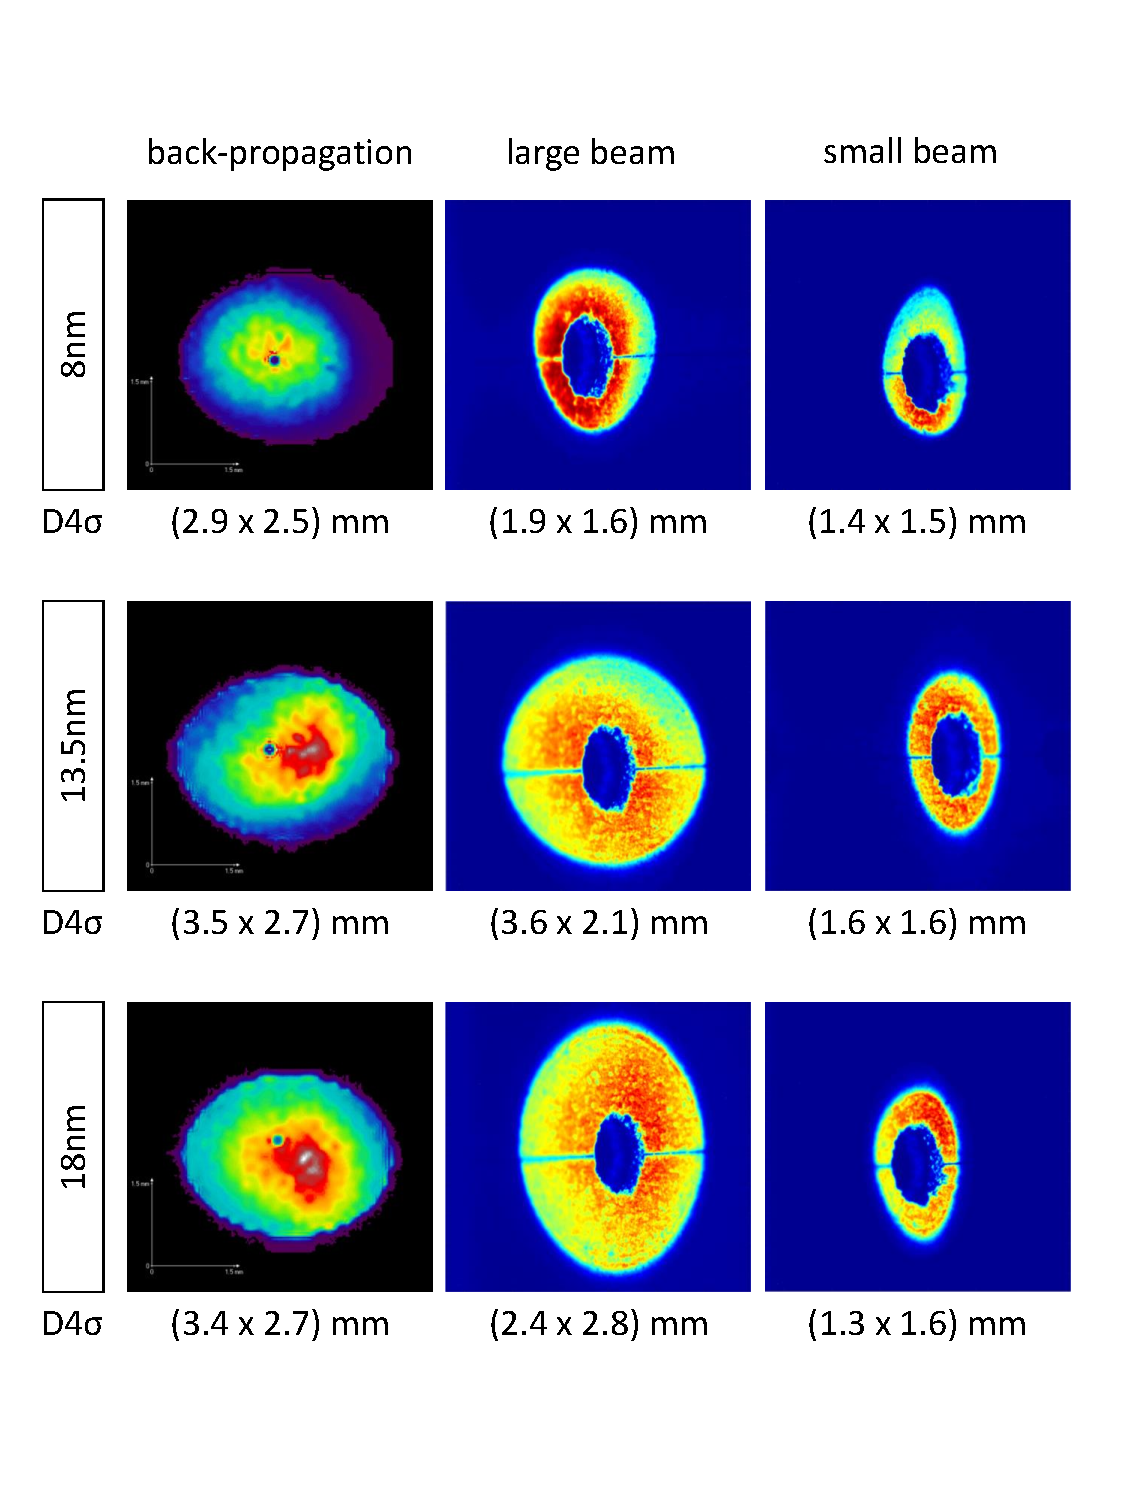
\includegraphics[width=0.8\textwidth]{gfx/beamprofiles.pdf}
    \caption{Beam profiles at the pinhole plate. The left column shows the back-propagation with MrBeam while the focus was set to be at the PMMA position, \SI{1067}{mm} upstream. The other two columns show image recorded of the fluorescent screen attached to the pinhole plate. The center column shows the beam with KAOS at the same configuration like in the left column, except for the \SI{8}{nm} acquisition.  The right column shows the images of KAOS configured such, that the beam size is approximately half as large. The corresponding beam widths in D4$\sigma$ (width $\times$ height) are displayed below each picture. The back-propagation images look in upstream direction, while the images of the fluorescent screen are facing downstream.}
    \label{fig:beamprofiles}
\end{figure}


\section{Analysis}

From the experimental geometry we calculate a scaled distance of $ z_M \approx 0.85 $ ( with $ z_p = \SI{6}{m} $ and $ z_0 = \SI{1}{m} $), $ \lambda = \SI{13.5}{nm} $ and $ w = \SI{10}{\micro\meter} $). Using equation (\ref{eq:cut-off}) this results in a cut-off value to apply Fraunhofer diffraction for the pinhole separation of $ D_\textup{cut-off} \approx \SI{20}{\micro\meter} $. All available pinhole separations are larger than this value, which means, that the central visibility cannot be used to determine the CDC $ \gamma $ and from its rms width the coherence length $\xi$.

Therefore, the deconvolution method has to be applied.


\section{Results and Discussion}

\subsection{Single-shot analysis}

\begin{figure}[htbp]
    \centering
    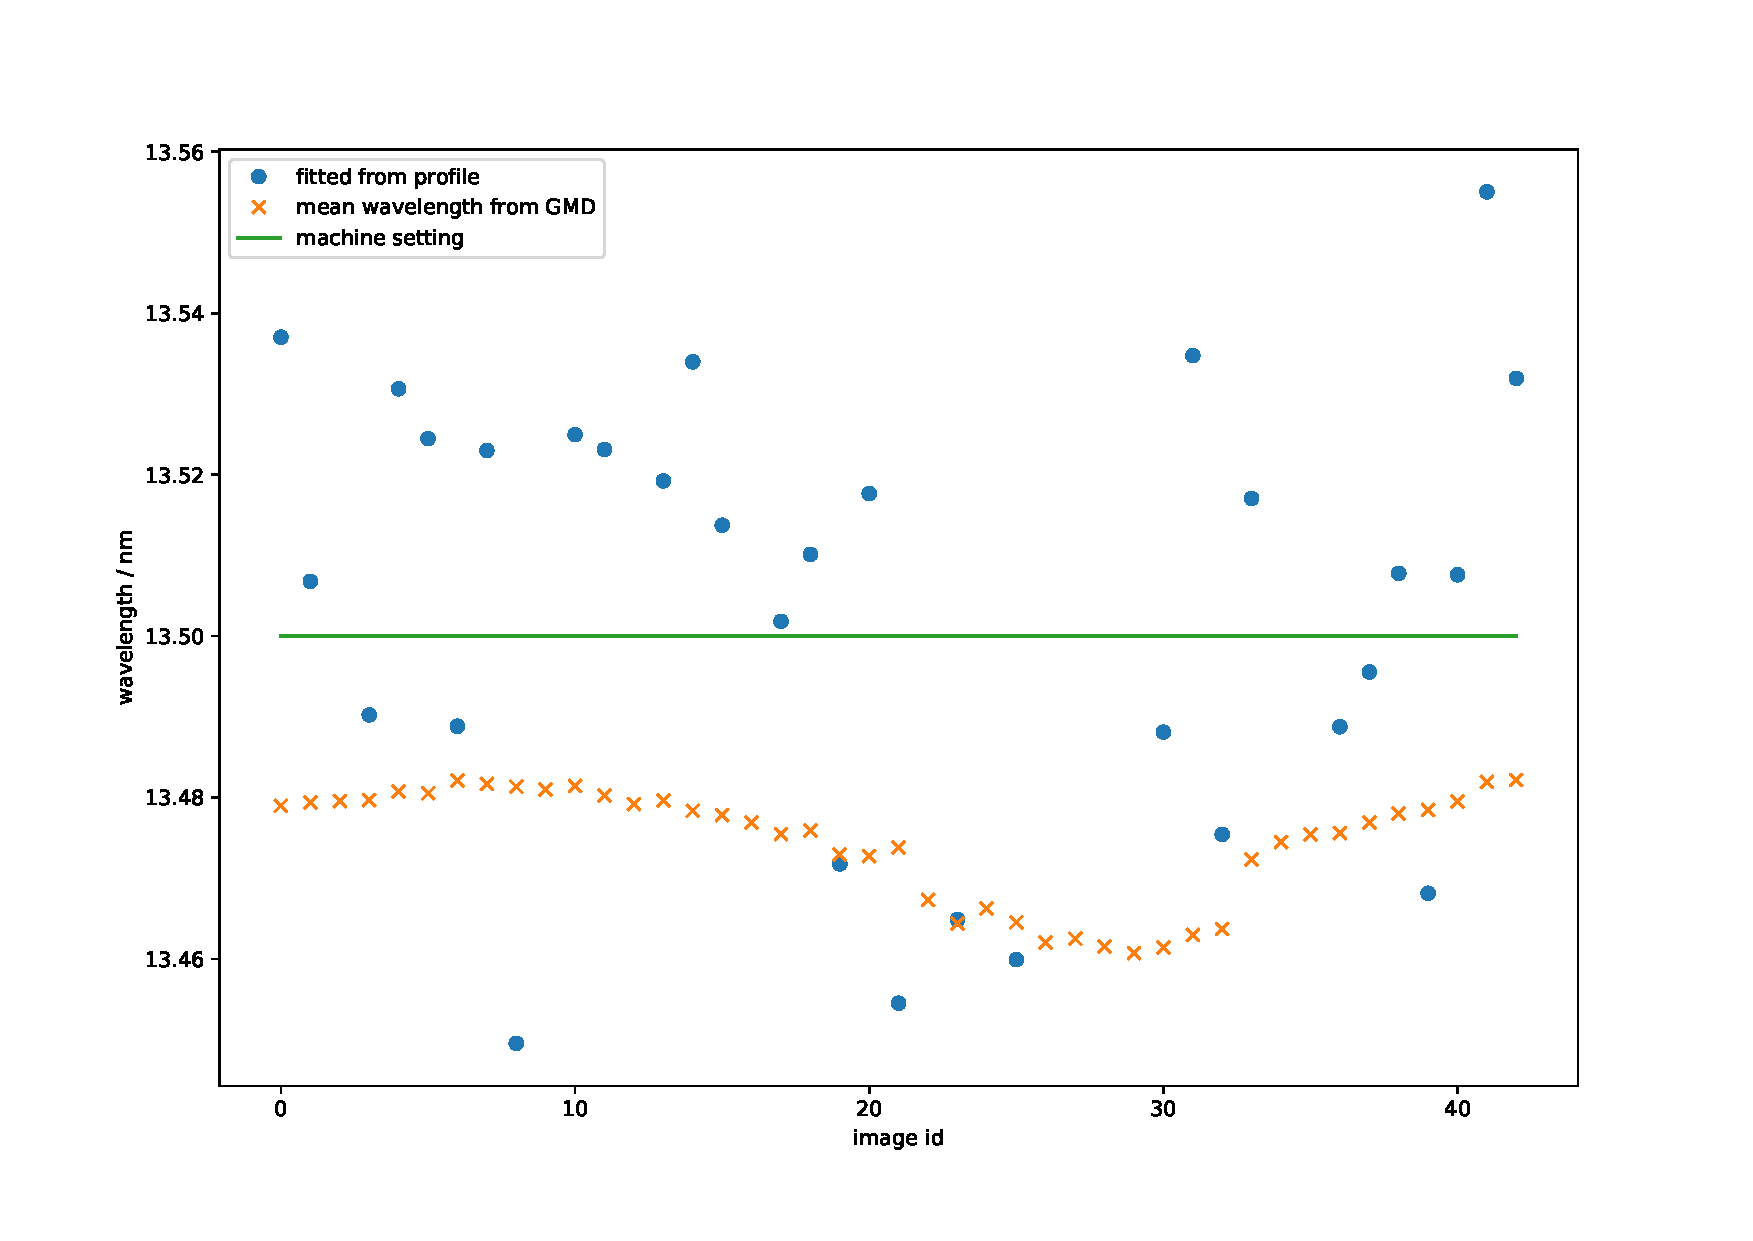
\includegraphics[width=0.7\textwidth]{gfx/13p5nm_S_445um/wavelength_FLASH2_USER1-2017-11-29T1007.pdf}
    \caption{Single-shot wavelength depending on the beam position. $\lambda=\SI{13.5}{nm}$, pinhole separation $d=\SI{445}{\micro\meter}$, orientation horizontal. rms width of the beam $\sigma_{\textup{Beam}} = \SI[separate-uncertainty=true]{405(20)}{\micro\meter}$}
    \label{fig:13p5nm_S_445um_wavelength_FLASH2_USER1-2017-11-29T1007}
\end{figure}

\begin{figure}[htbp]
    \centering
    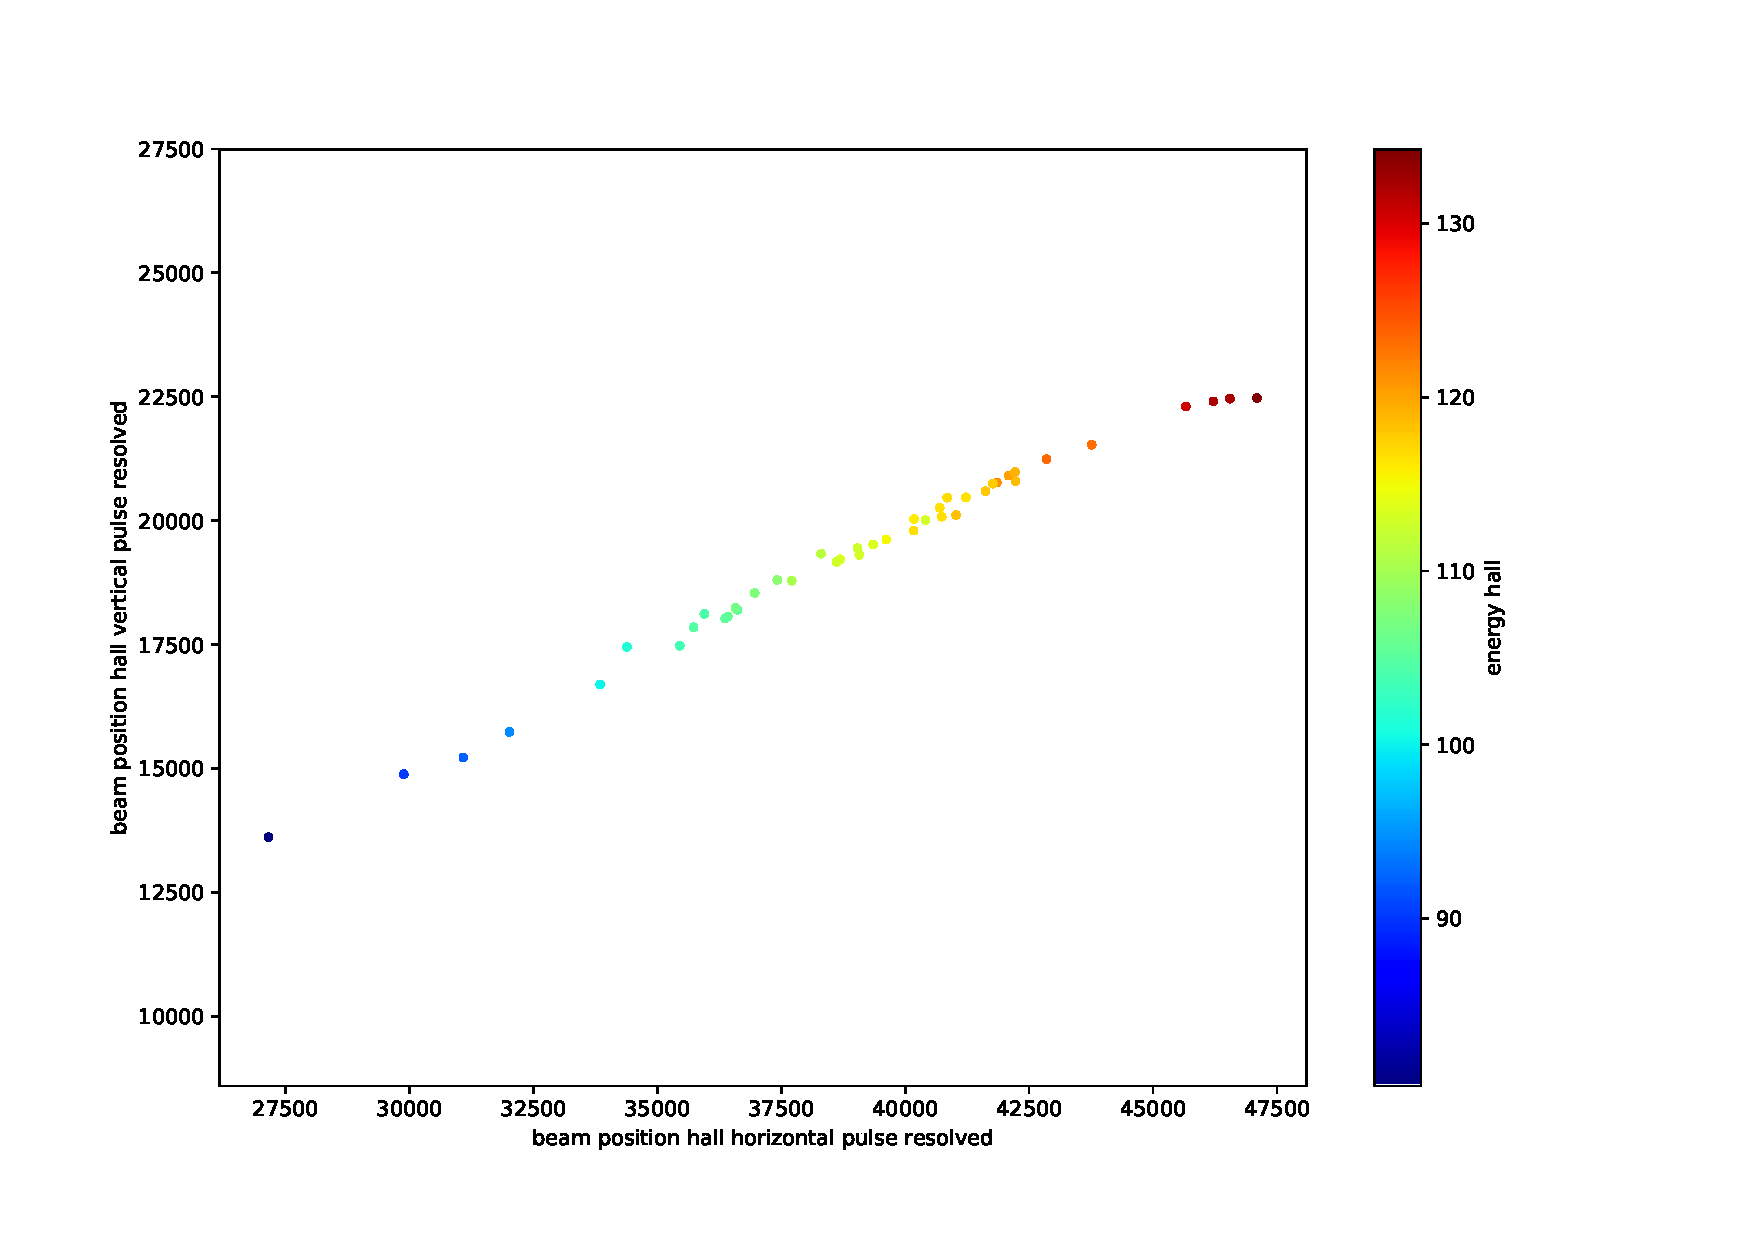
\includegraphics[width=0.7\textwidth]{gfx/13p5nm_S_445um/energy_vs_position_FLASH2_USER1-2017-11-29T1007.pdf}
    \caption{Single-shot coherence energy depending on the beam position. $\lambda=\SI{13.5}{nm}$, pinhole separation $d=\SI{445}{\micro\meter}$, orientation horizontal. rms width of the beam $\sigma_{\textup{Beam}} = \SI[separate-uncertainty=true]{405(20)}{\micro\meter}$}
    \label{fig:13p5nm_S_445um_energy_vs_position_FLASH2_USER1-2017-11-29T1007}
\end{figure}

\begin{figure}[htbp]
    \centering
    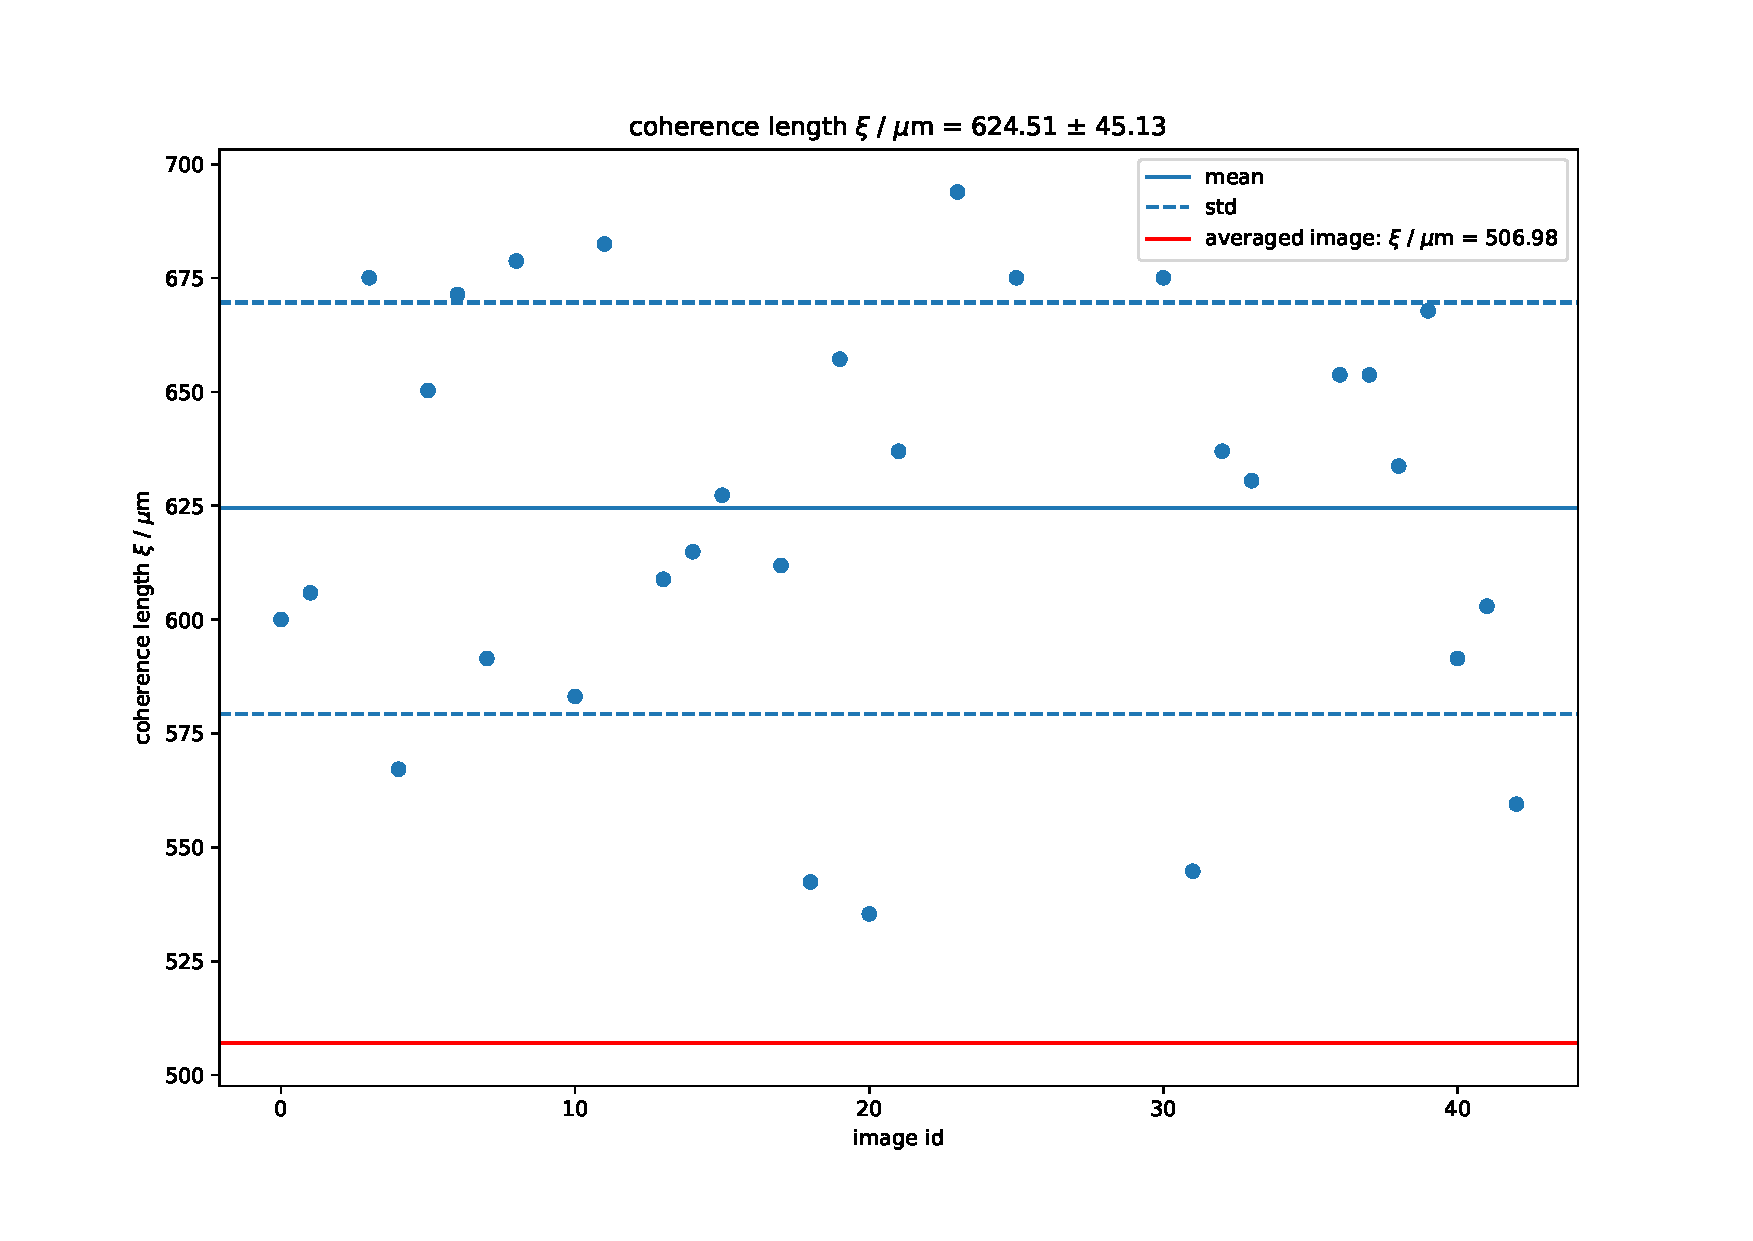
\includegraphics[width=0.7\textwidth]{gfx/13p5nm_S_445um/coherencelength_FLASH2_USER1-2017-11-29T1007.pdf}
    \caption{Single-shot coherence length $\xi$ calculation by applying the deconvolution-method. $\lambda=\SI{13.5}{nm}$, pinhole separation $d=\SI{445}{\micro\meter}$, orientation horizontal. rms width of the beam $\sigma_{\textup{Beam}} = \SI[separate-uncertainty=true]{405(20)}{\micro\meter}$}
    \label{fig:13p5nm_S_445um_coherencelength_FLASH2_USER1-2017-11-29T1007}
\end{figure}

\begin{figure}[htbp]
    \centering
    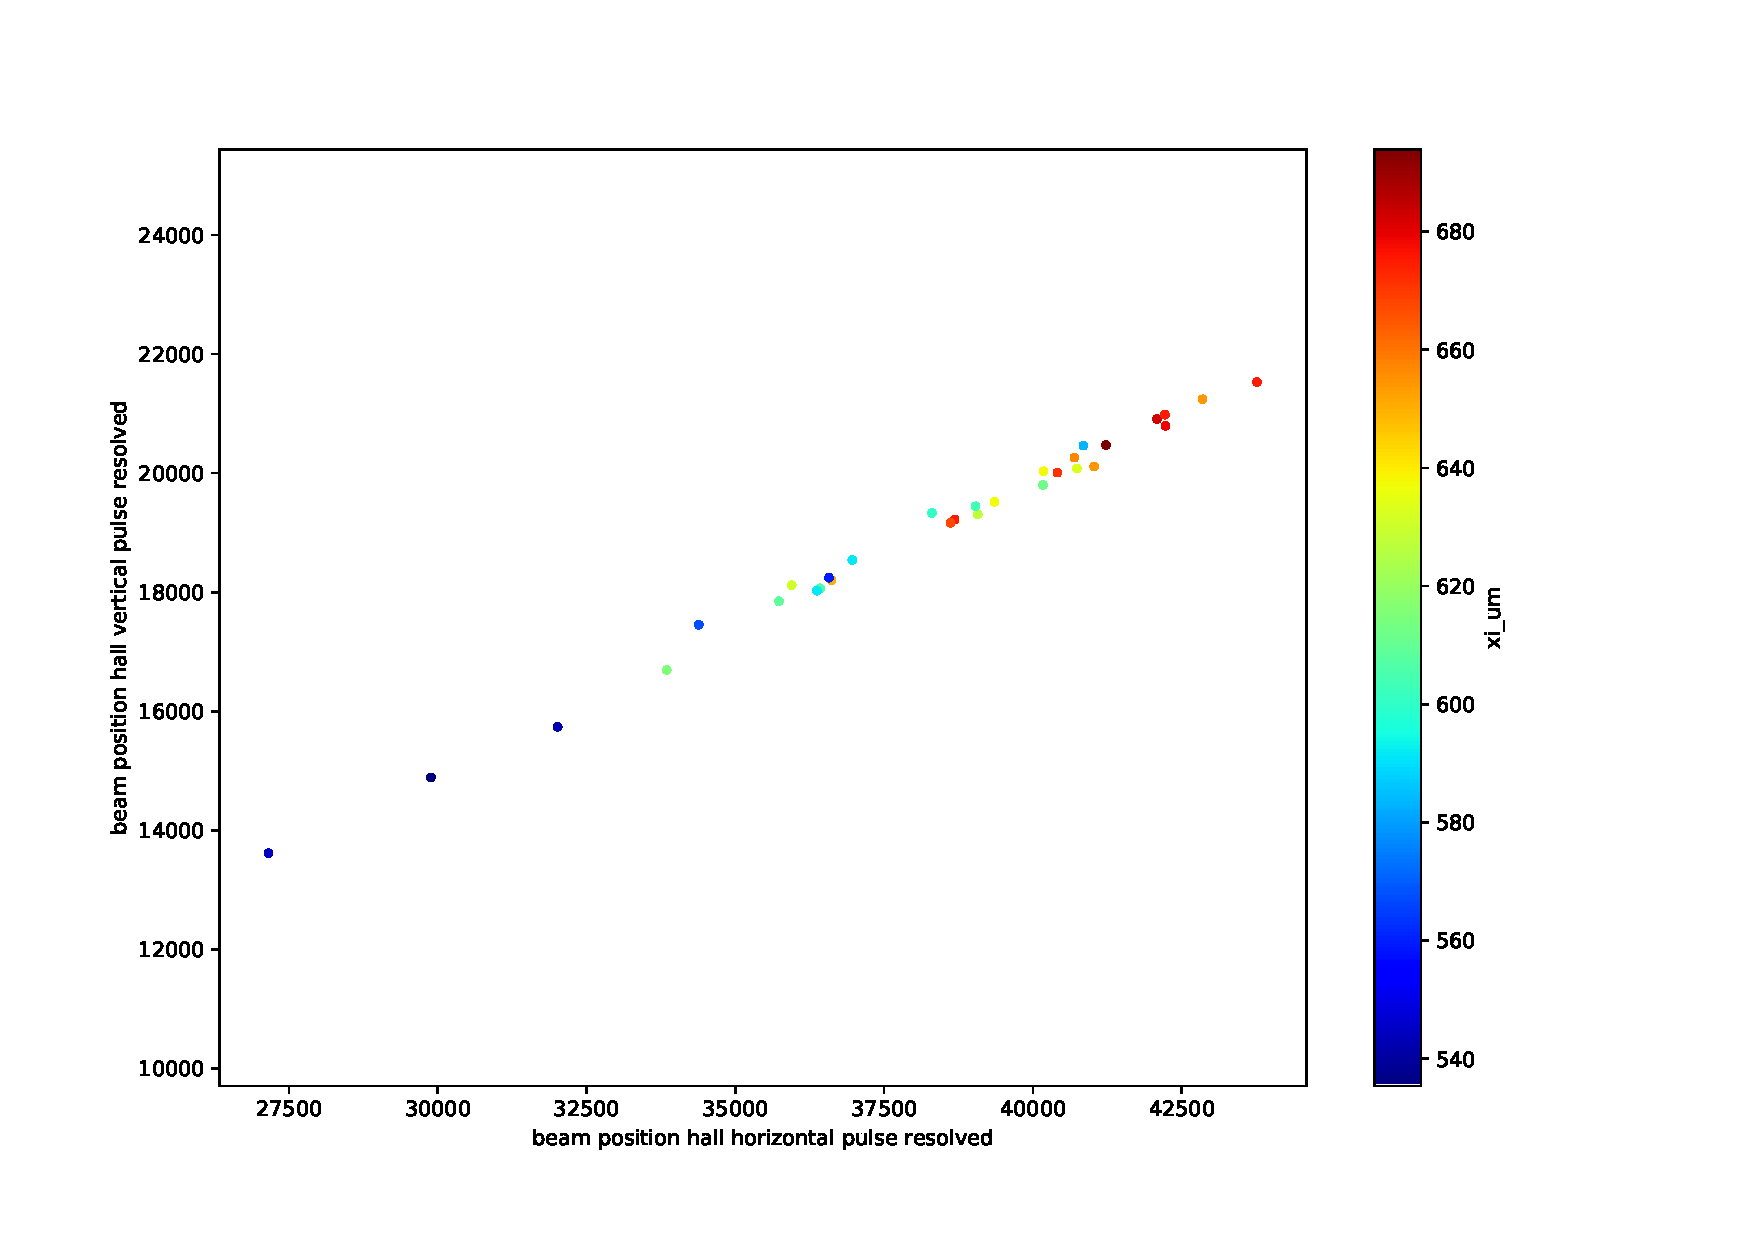
\includegraphics[width=0.7\textwidth]{gfx/13p5nm_S_445um/coherencelength_vs_position_FLASH2_USER1-2017-11-29T1007.pdf}
    \caption{Single-shot coherence length $\xi$ depending on the beam position. $\lambda=\SI{13.5}{nm}$, pinhole separation $d=\SI{445}{\micro\meter}$, orientation horizontal. rms width of the beam $\sigma_{\textup{Beam}} = \SI[separate-uncertainty=true]{405(20)}{\micro\meter}$}
    \label{fig:13p5nm_S_445um_coherencelength_vs_position_FLASH2_USER1-2017-11-29T1007}
\end{figure}

\begin{figure}[htbp]
    \centering
    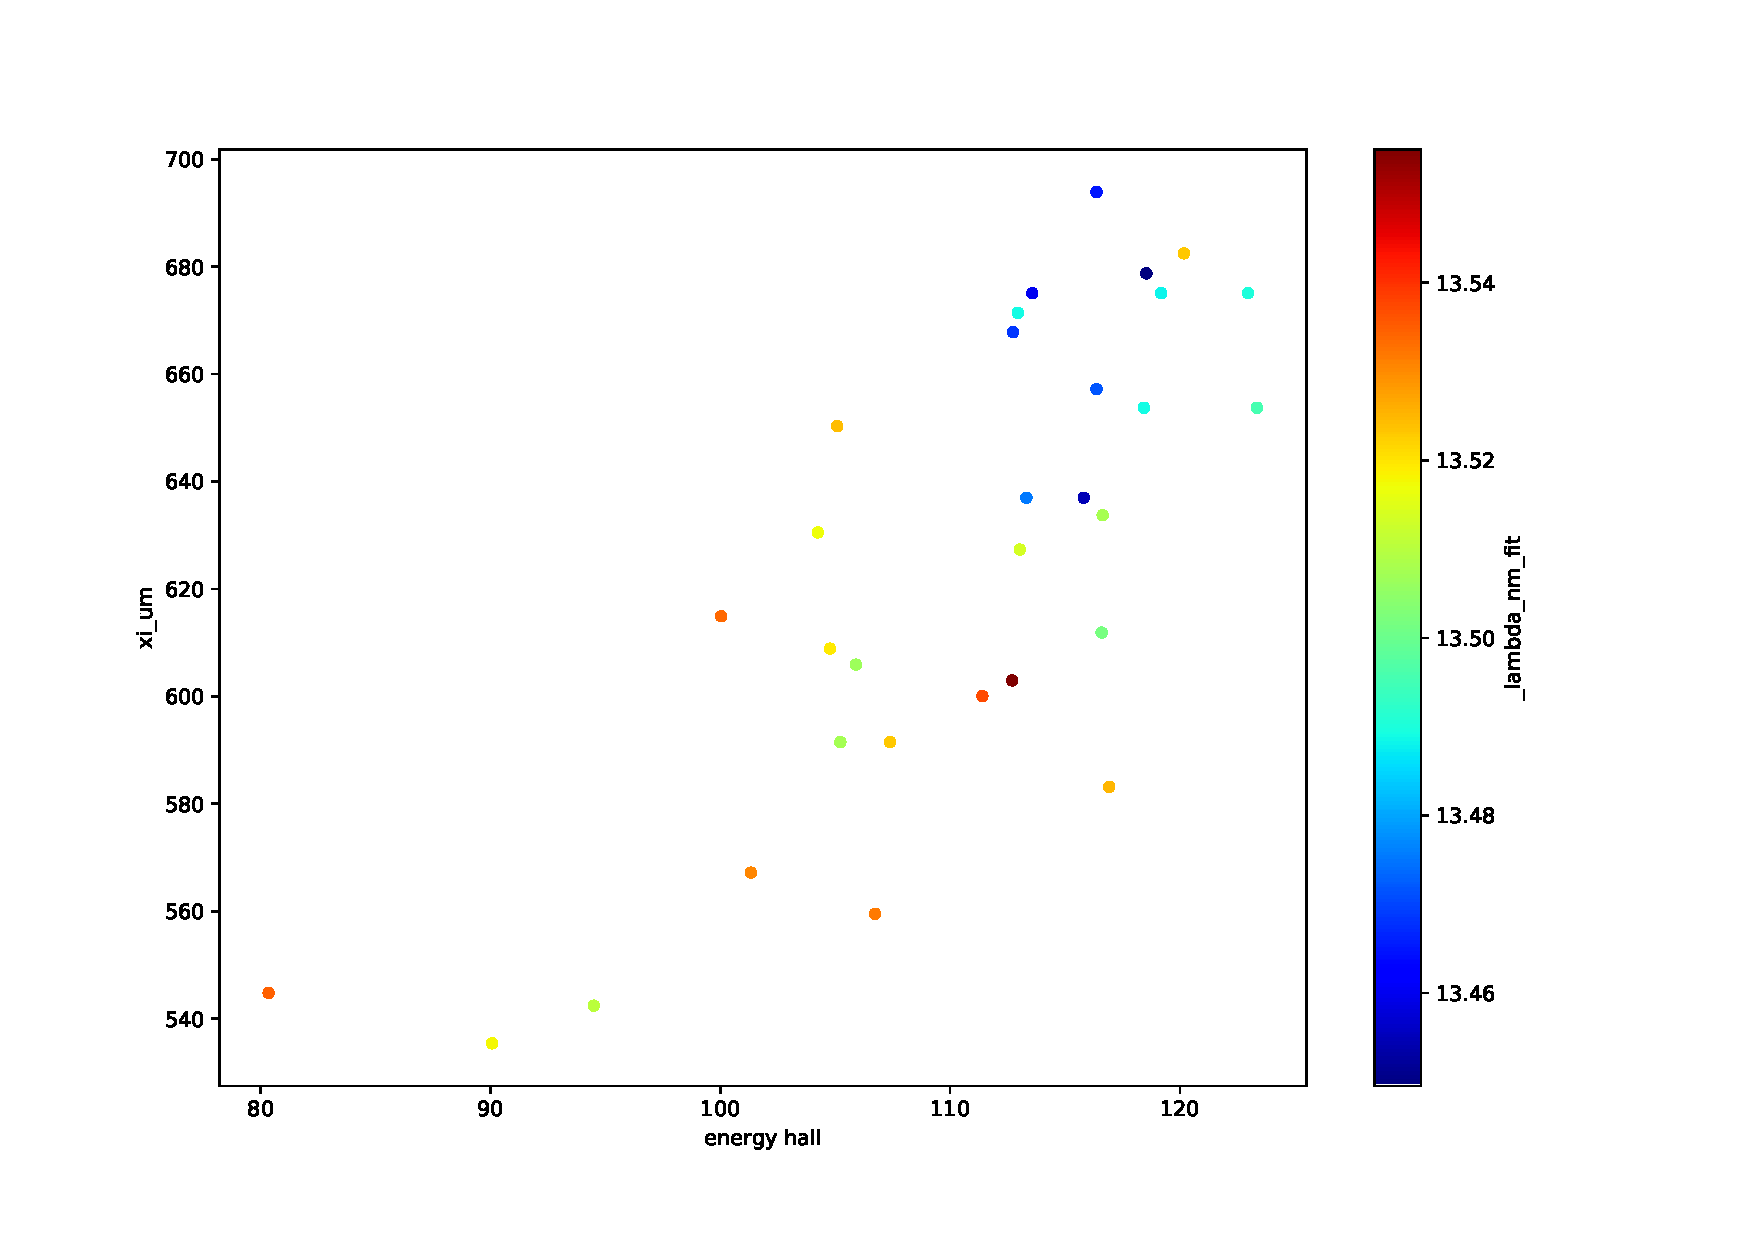
\includegraphics[width=0.7\textwidth]{gfx/13p5nm_S_445um/xi_um_vs_energy_hall_FLASH2_USER1-2017-11-29T1007.pdf}
    \caption{Coherence length depending on the beam energy. $\lambda=\SI{13.5}{nm}$, pinhole separation $d=\SI{445}{\micro\meter}$, orientation horizontal. rms width of the beam $\sigma_{\textup{Beam}} = \SI[separate-uncertainty=true]{405(20)}{\micro\meter}$}
    \label{fig:13p5nm_S_445um_xi_um_vs_energy_hall_FLASH2_USER1-2017-11-29T1007}
\end{figure}

\begin{figure}[htbp]
    \centering
    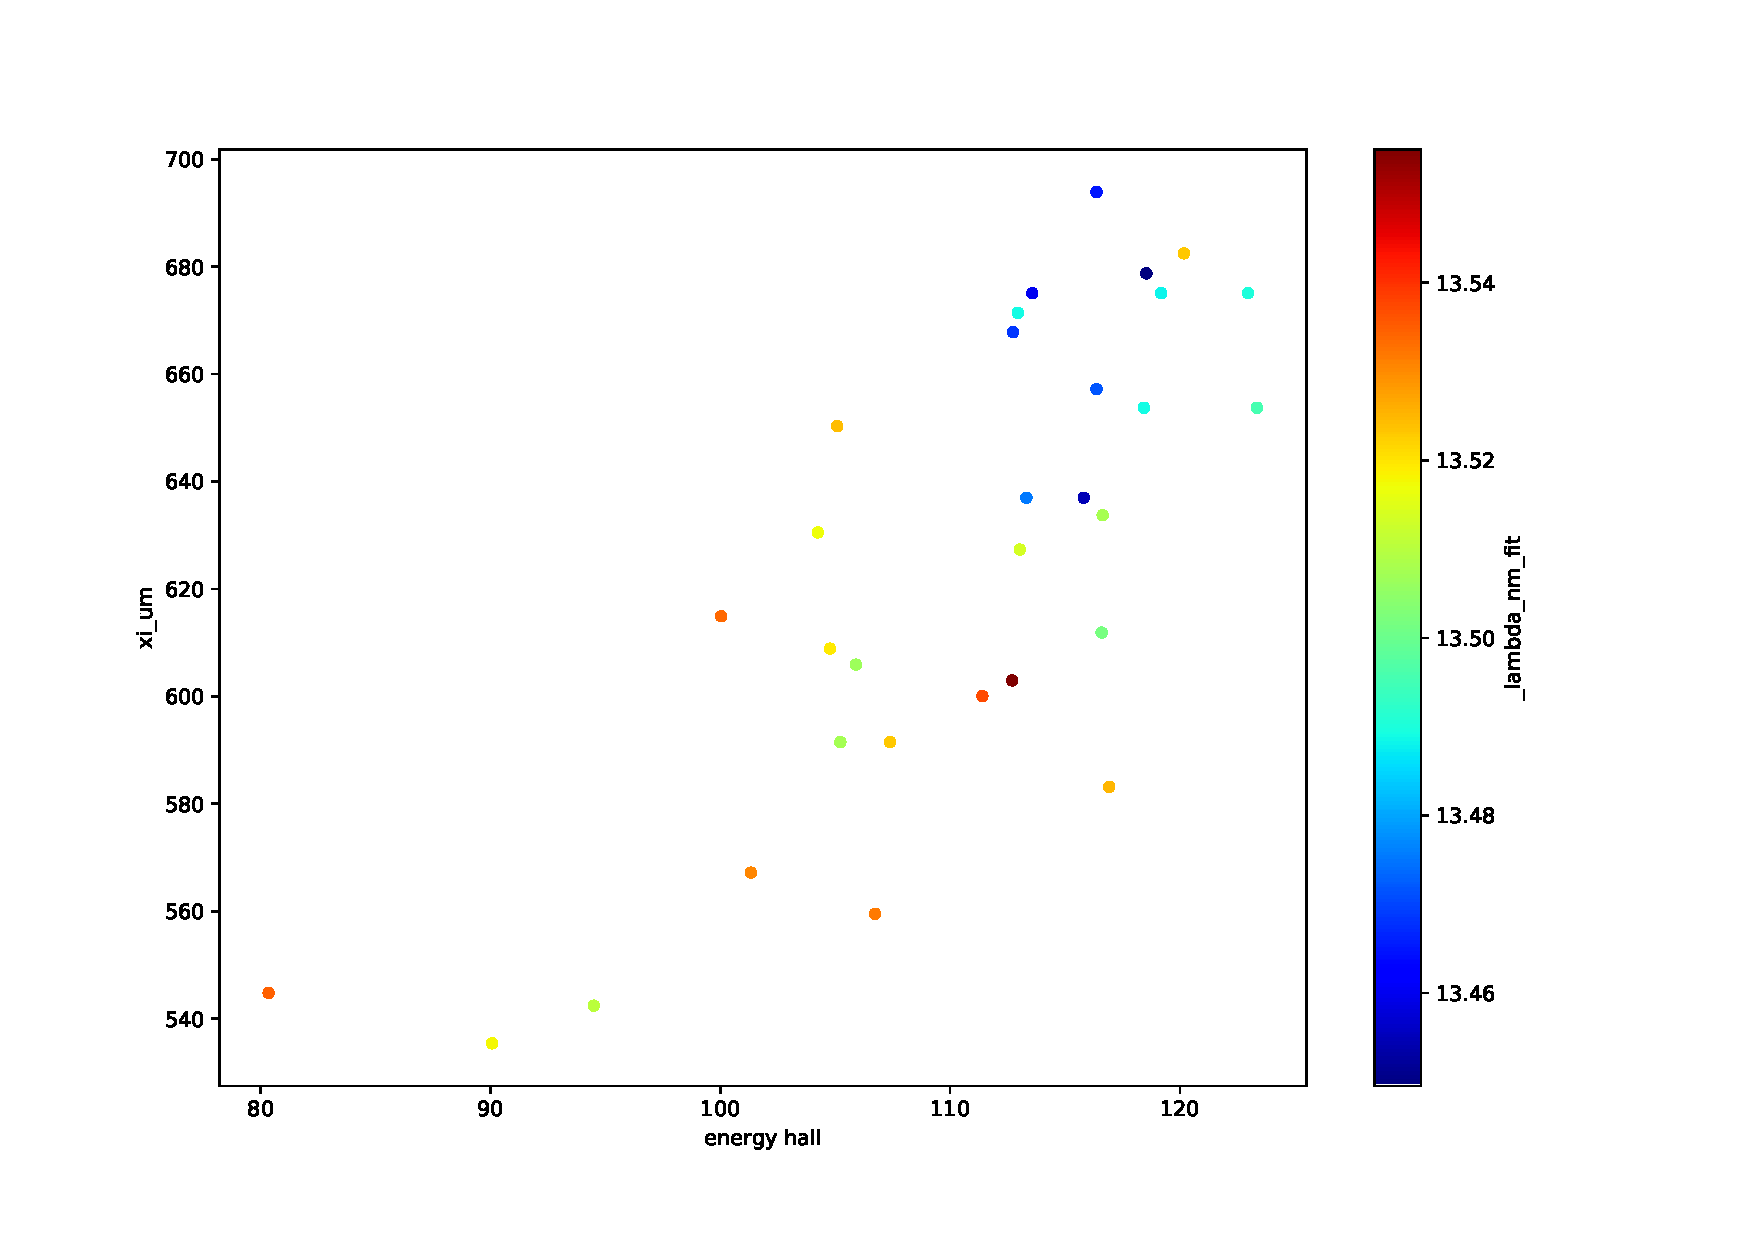
\includegraphics[width=0.7\textwidth]{gfx/13p5nm_S_445um/xi_um_vs_energy_hall_FLASH2_USER1-2017-11-29T1007.pdf}
    \caption{Coherence length depending on the wavelength!!!. $\lambda=\SI{13.5}{nm}$, pinhole separation $d=\SI{445}{\micro\meter}$, orientation horizontal. rms width of the beam $\sigma_{\textup{Beam}} = \SI[separate-uncertainty=true]{405(20)}{\micro\meter}$}
    \label{fig:13p5nm_S_445um_xi_um_vs_energy_hall_FLASH2_USER1-2017-11-29T1007}
\end{figure}

\begin{figure}[htbp]

	\begin{subfigure}{.4\linewidth}
	    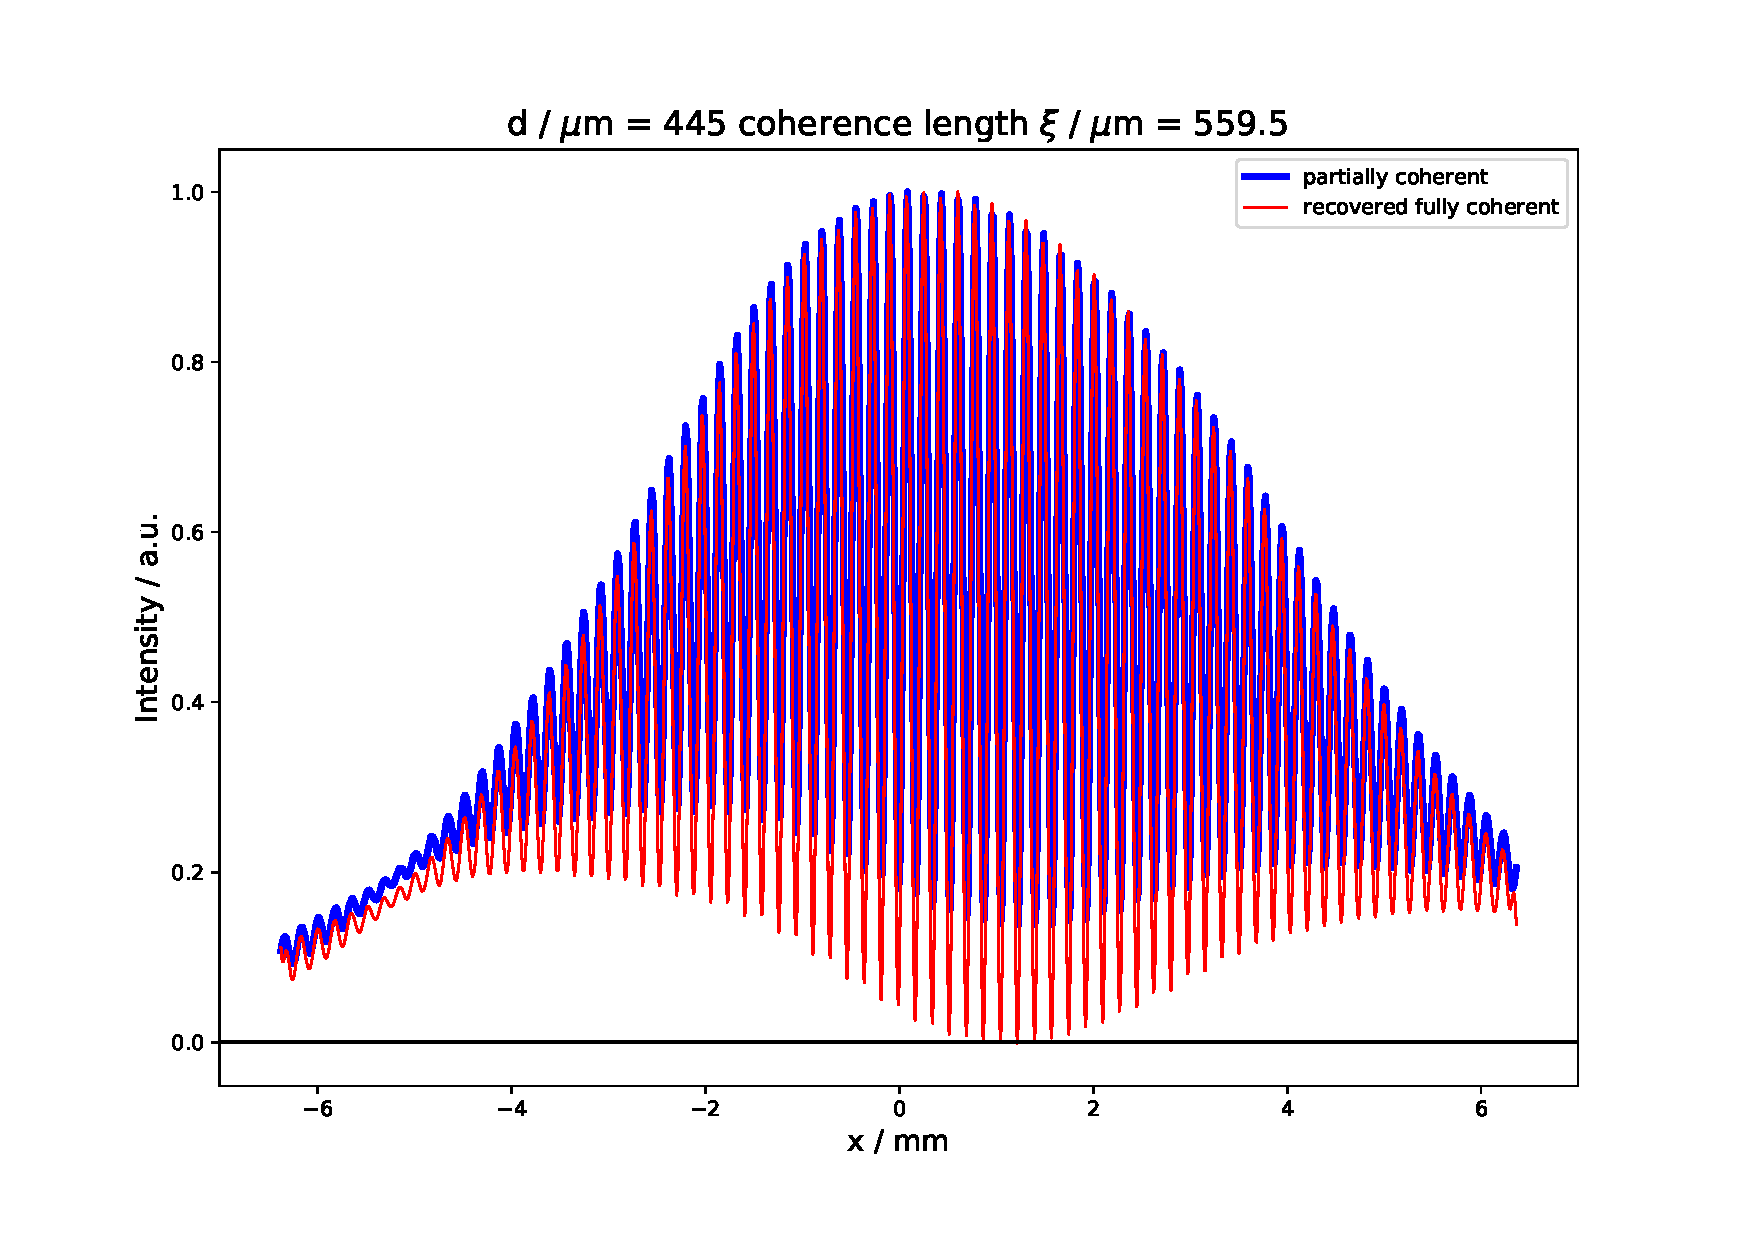
\includegraphics[width=0.5\textwidth]{gfx/13p5nm_S_445um/profile36.pdf}
	\end{subfigure}
	\begin{subfigure}{.4\linewidth}
	    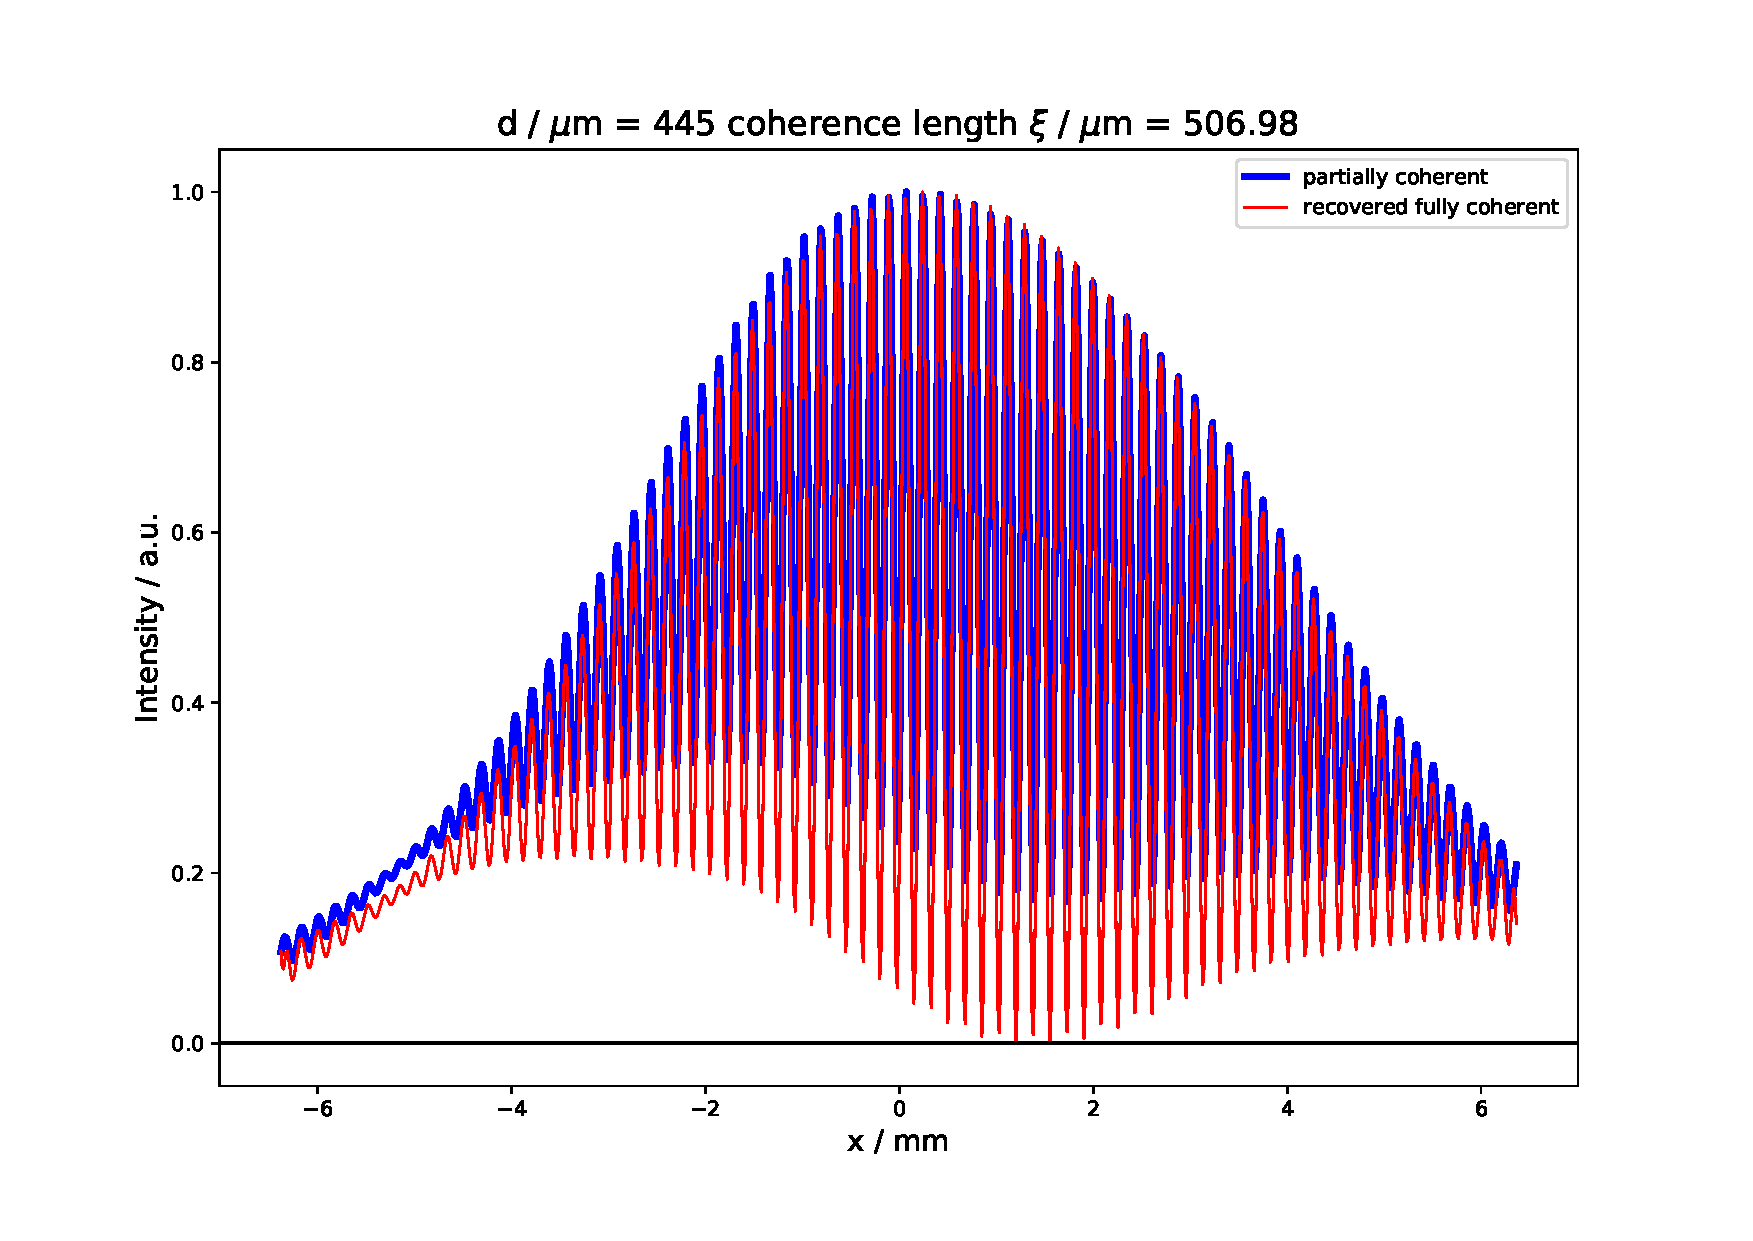
\includegraphics[width=0.5\textwidth]{gfx/13p5nm_S_445um/profile50.pdf}
	\end{subfigure}
	\begin{subfigure}{.4\linewidth}
	    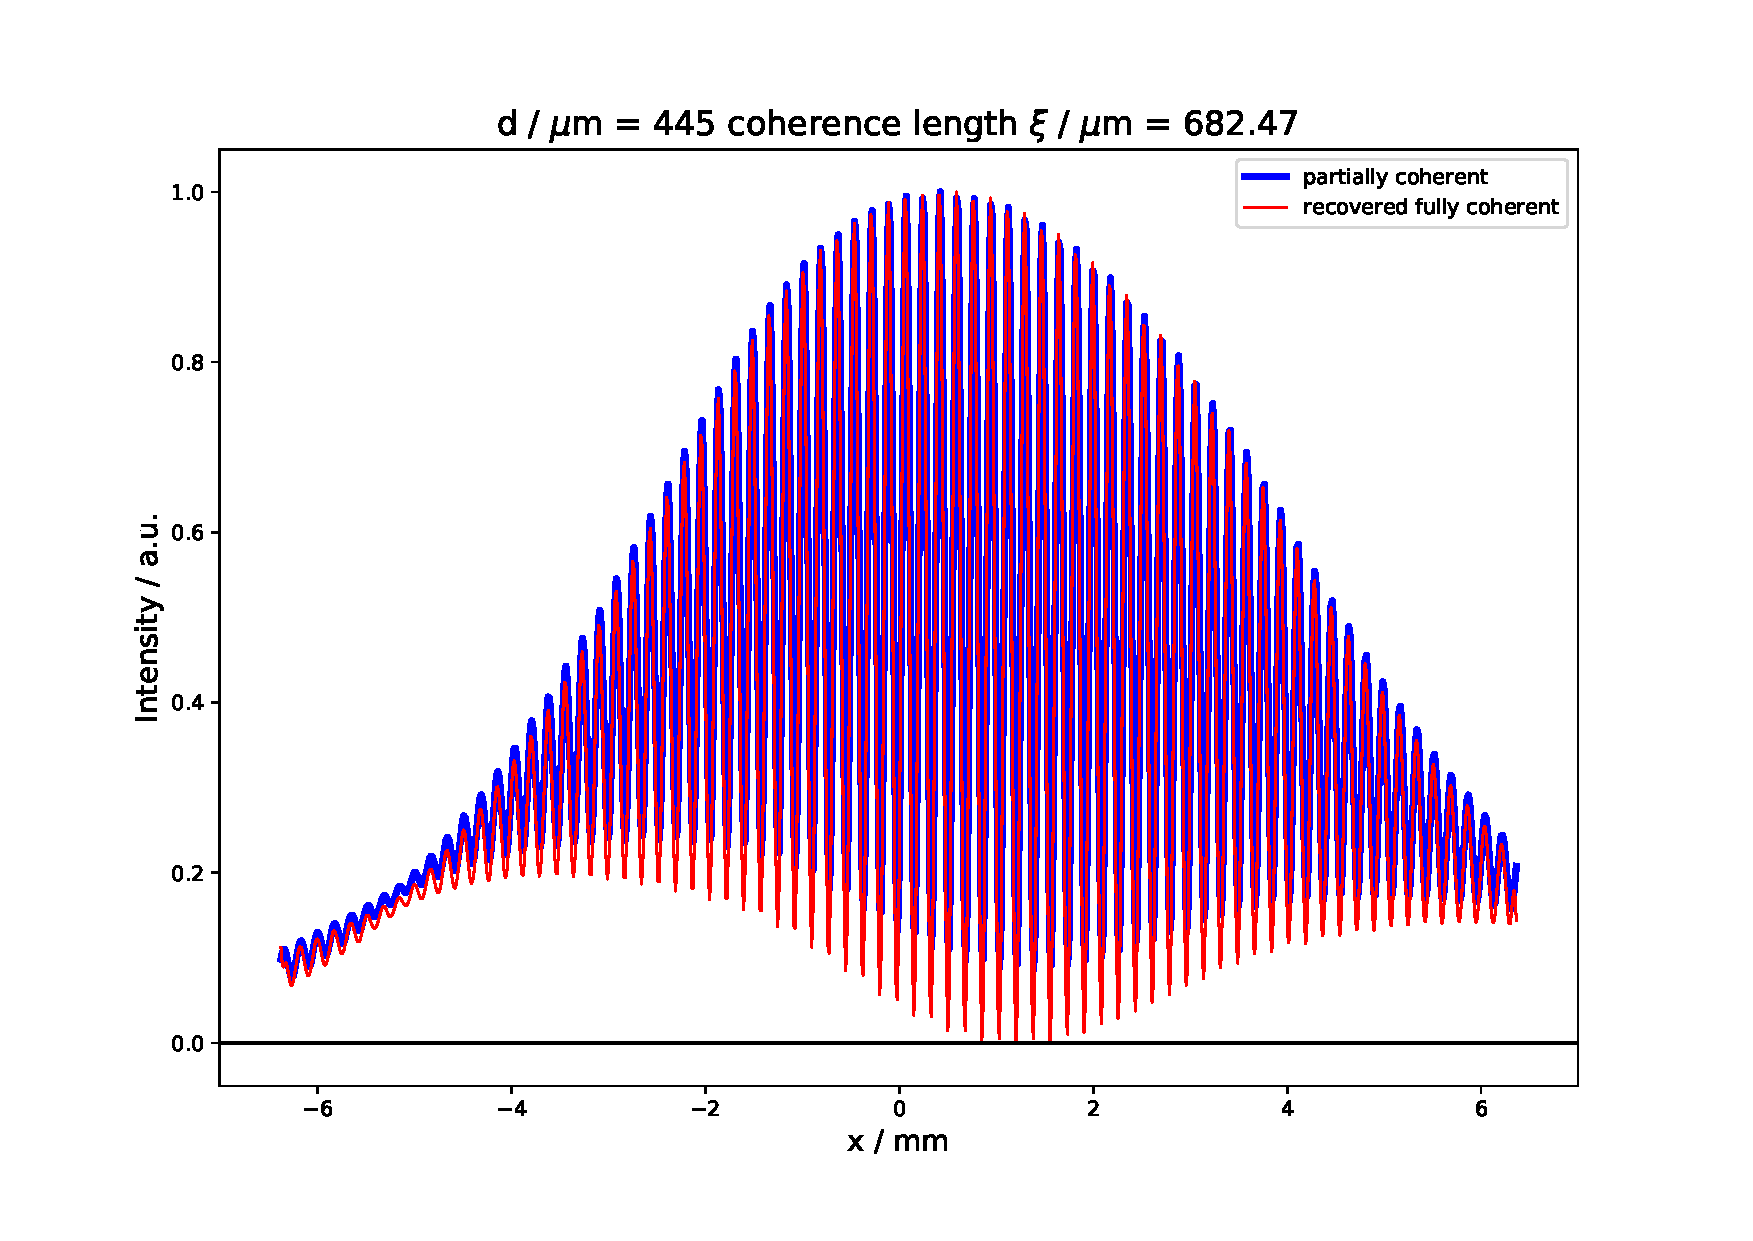
\includegraphics[width=0.5\textwidth]{gfx/13p5nm_S_445um/profile32.pdf}	
	\end{subfigure}
	\begin{subfigure}{.4\linewidth}
    	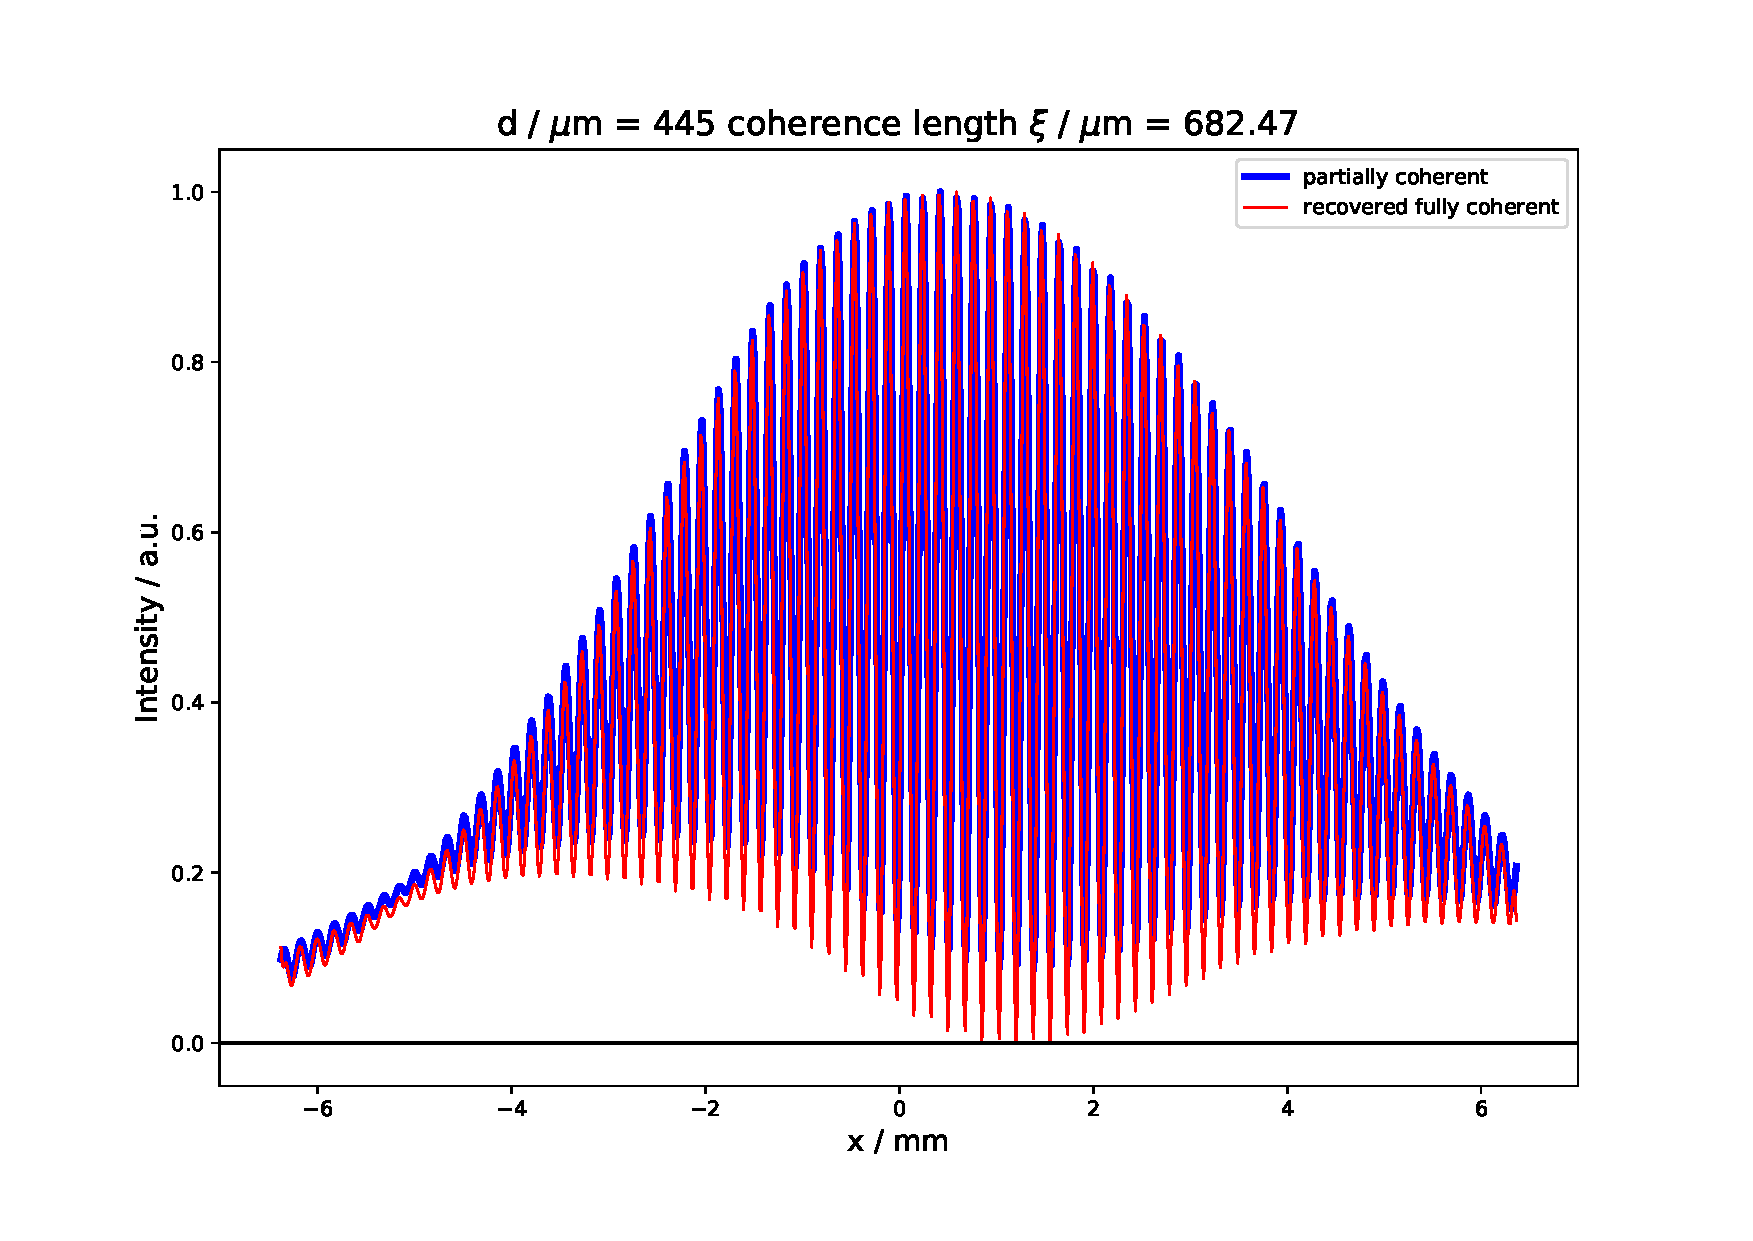
\includegraphics[width=0.5\textwidth]{gfx/13p5nm_S_445um/profile32.pdf}
	\end{subfigure}
\end{figure}



\subsection{beam and wave front stability}




\subsection{coherence}
\begin{figure}[hbtp]
    \centering
    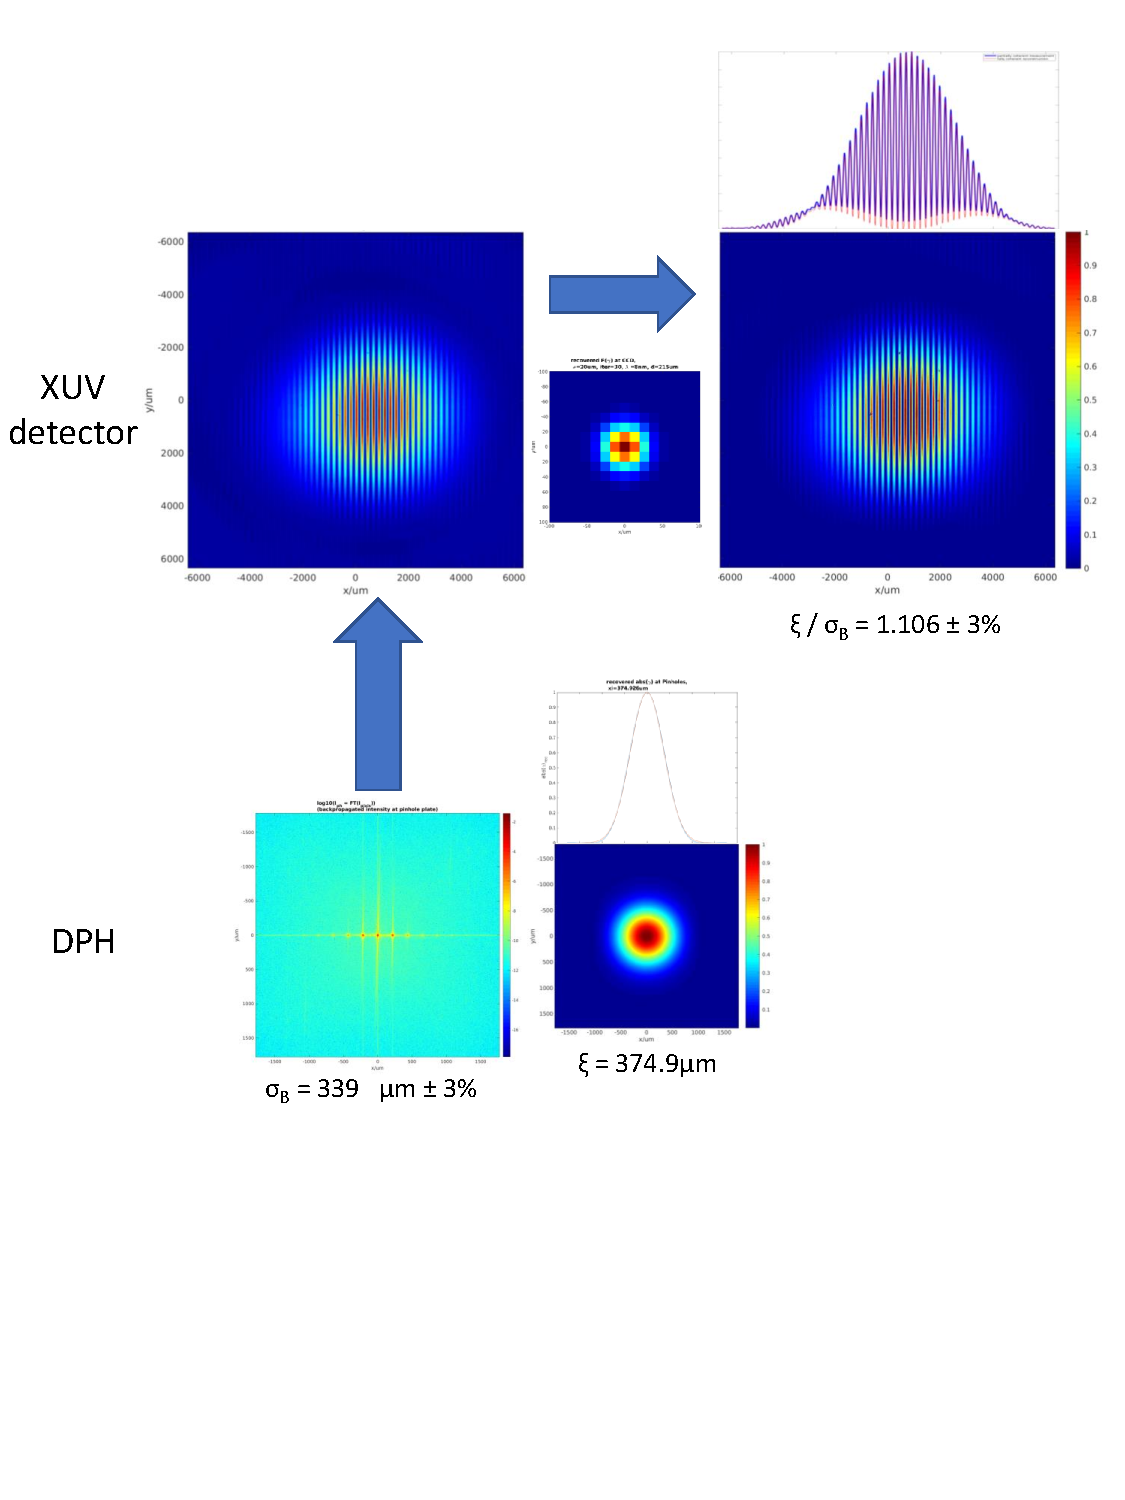
\includegraphics[width=0.9\textwidth]{gfx/deconvolution_example_8nm_215_hor.pdf}
    \caption{Determination of the coherence length $\xi$ by applying the deconvolution-method. $\lambda=\SI{8}{nm}$, pinhole separation $d=\SI{215}{\micro\meter}$, orientation horizontal.}
    \label{fig:deconvolution_example_8nm_215_hor}
\end{figure}

\begin{figure}[hbtp]
    \centering
    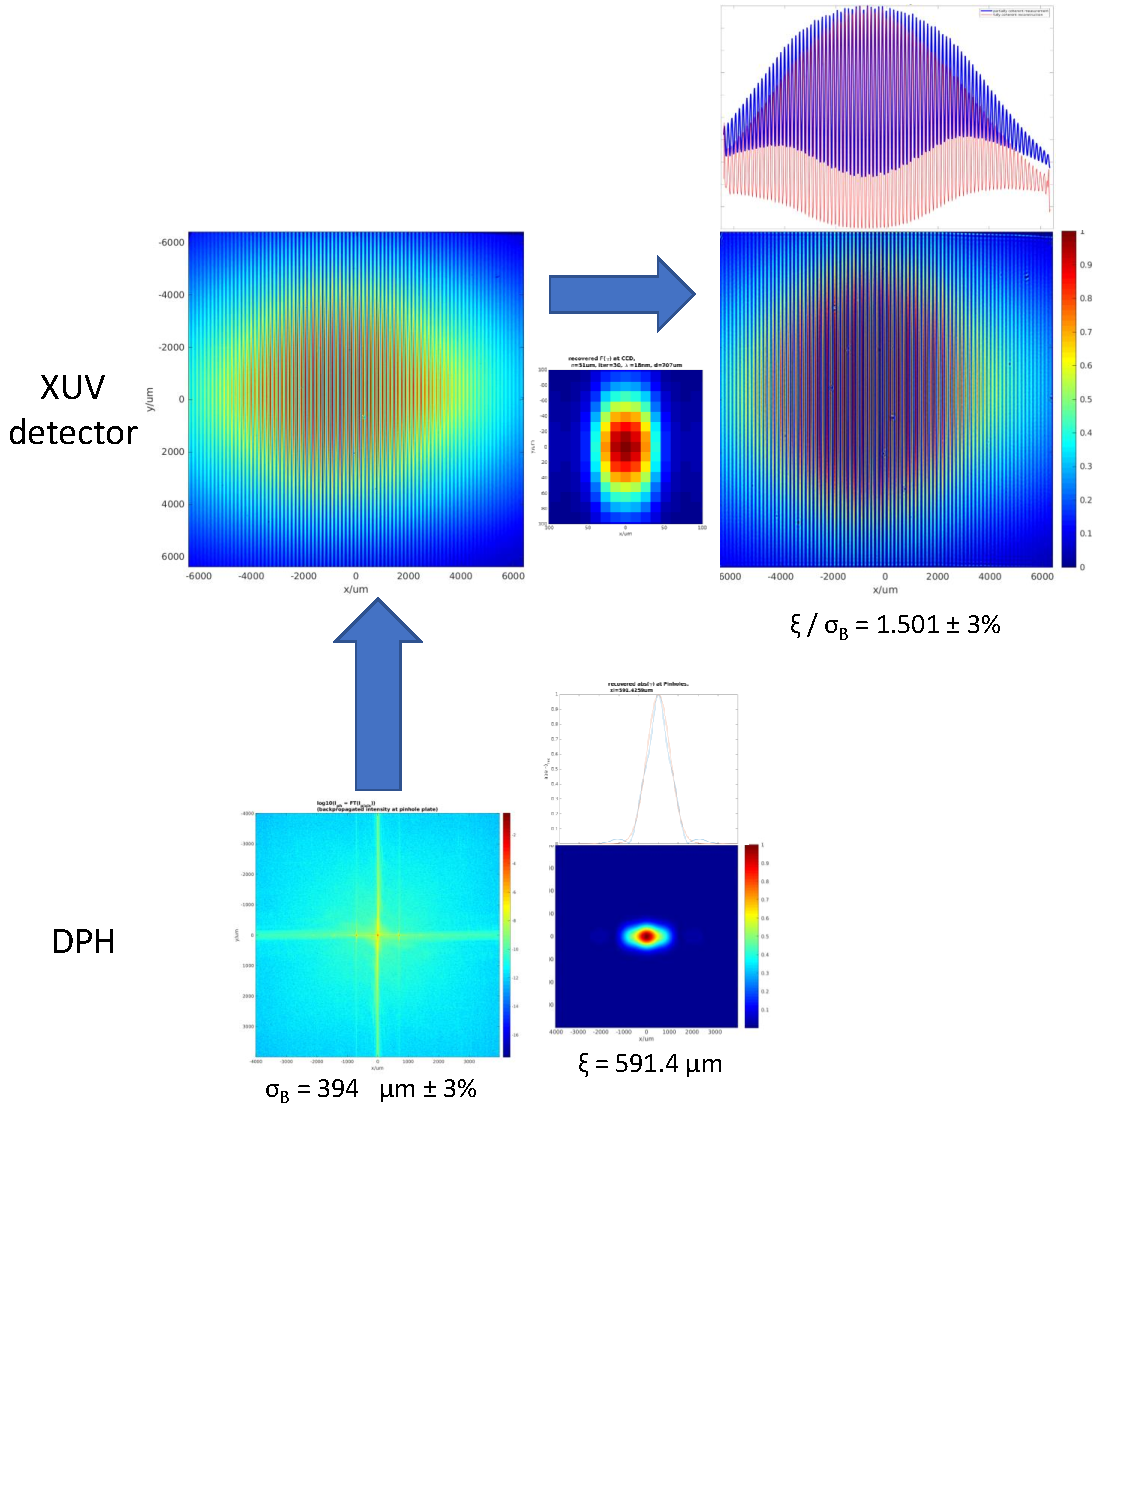
\includegraphics[width=0.9\textwidth]{gfx/deconvolution_example_18nm_707_ver_S.pdf}
    \caption{Determination of the coherence length $\xi$ by applying the deconvolution-method. $\lambda=\SI{18}{nm}$, pinhole separation $d=\SI{707}{\micro\meter}$, orientation vertical.}
    \label{fig:deconvolution_example_18nm_707_ver_S}
\end{figure}


\begin{figure}[hbtp]
    \centering
    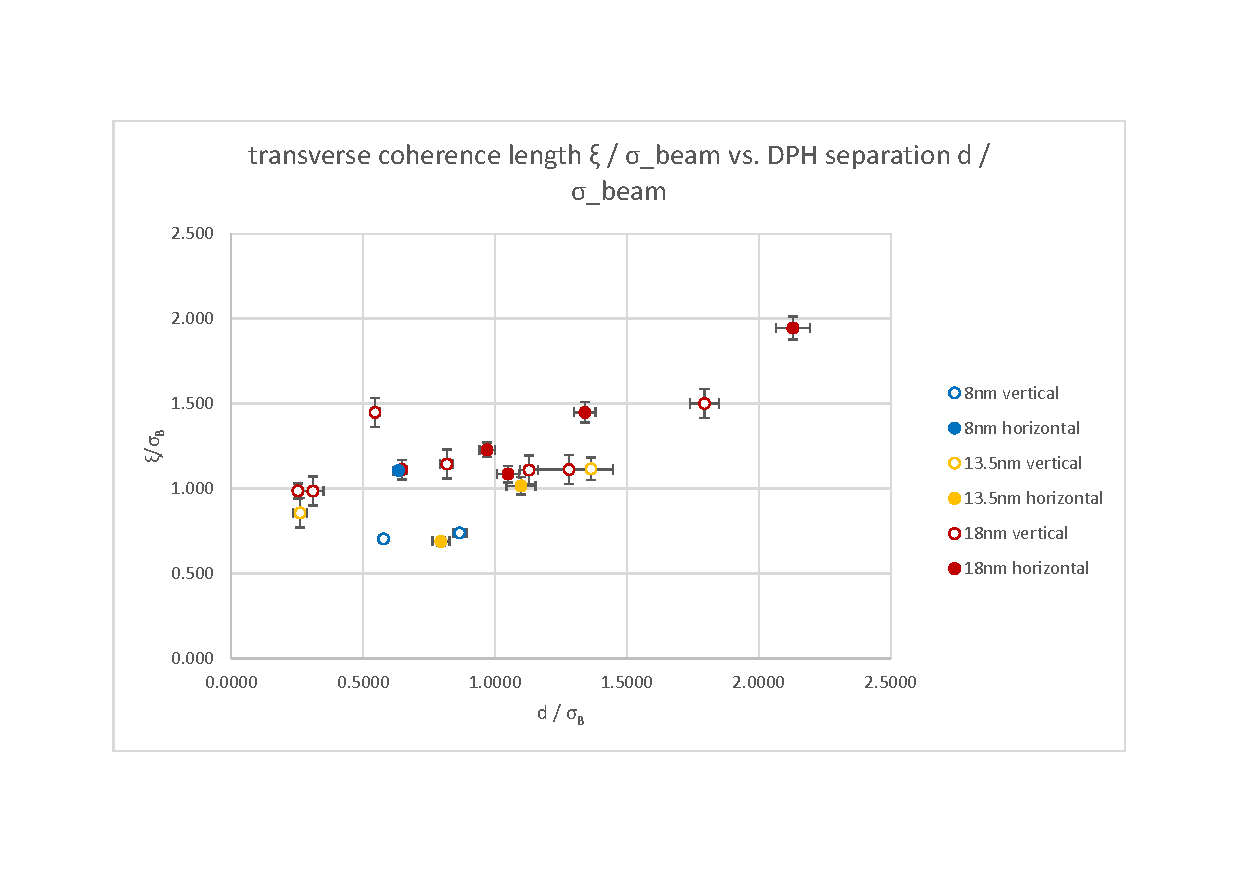
\includegraphics[width=1\textwidth]{gfx/DPH_results_coherence_vs_separation.pdf}
    \caption{Coherence length in relation to the pinhole separation determined from averaged-shots analysis using blinr-deconvolution method.}
    \label{fig:DPH_results_coherence_vs_separation}
\end{figure}

\begin{figure}[hbtp]
    \centering
    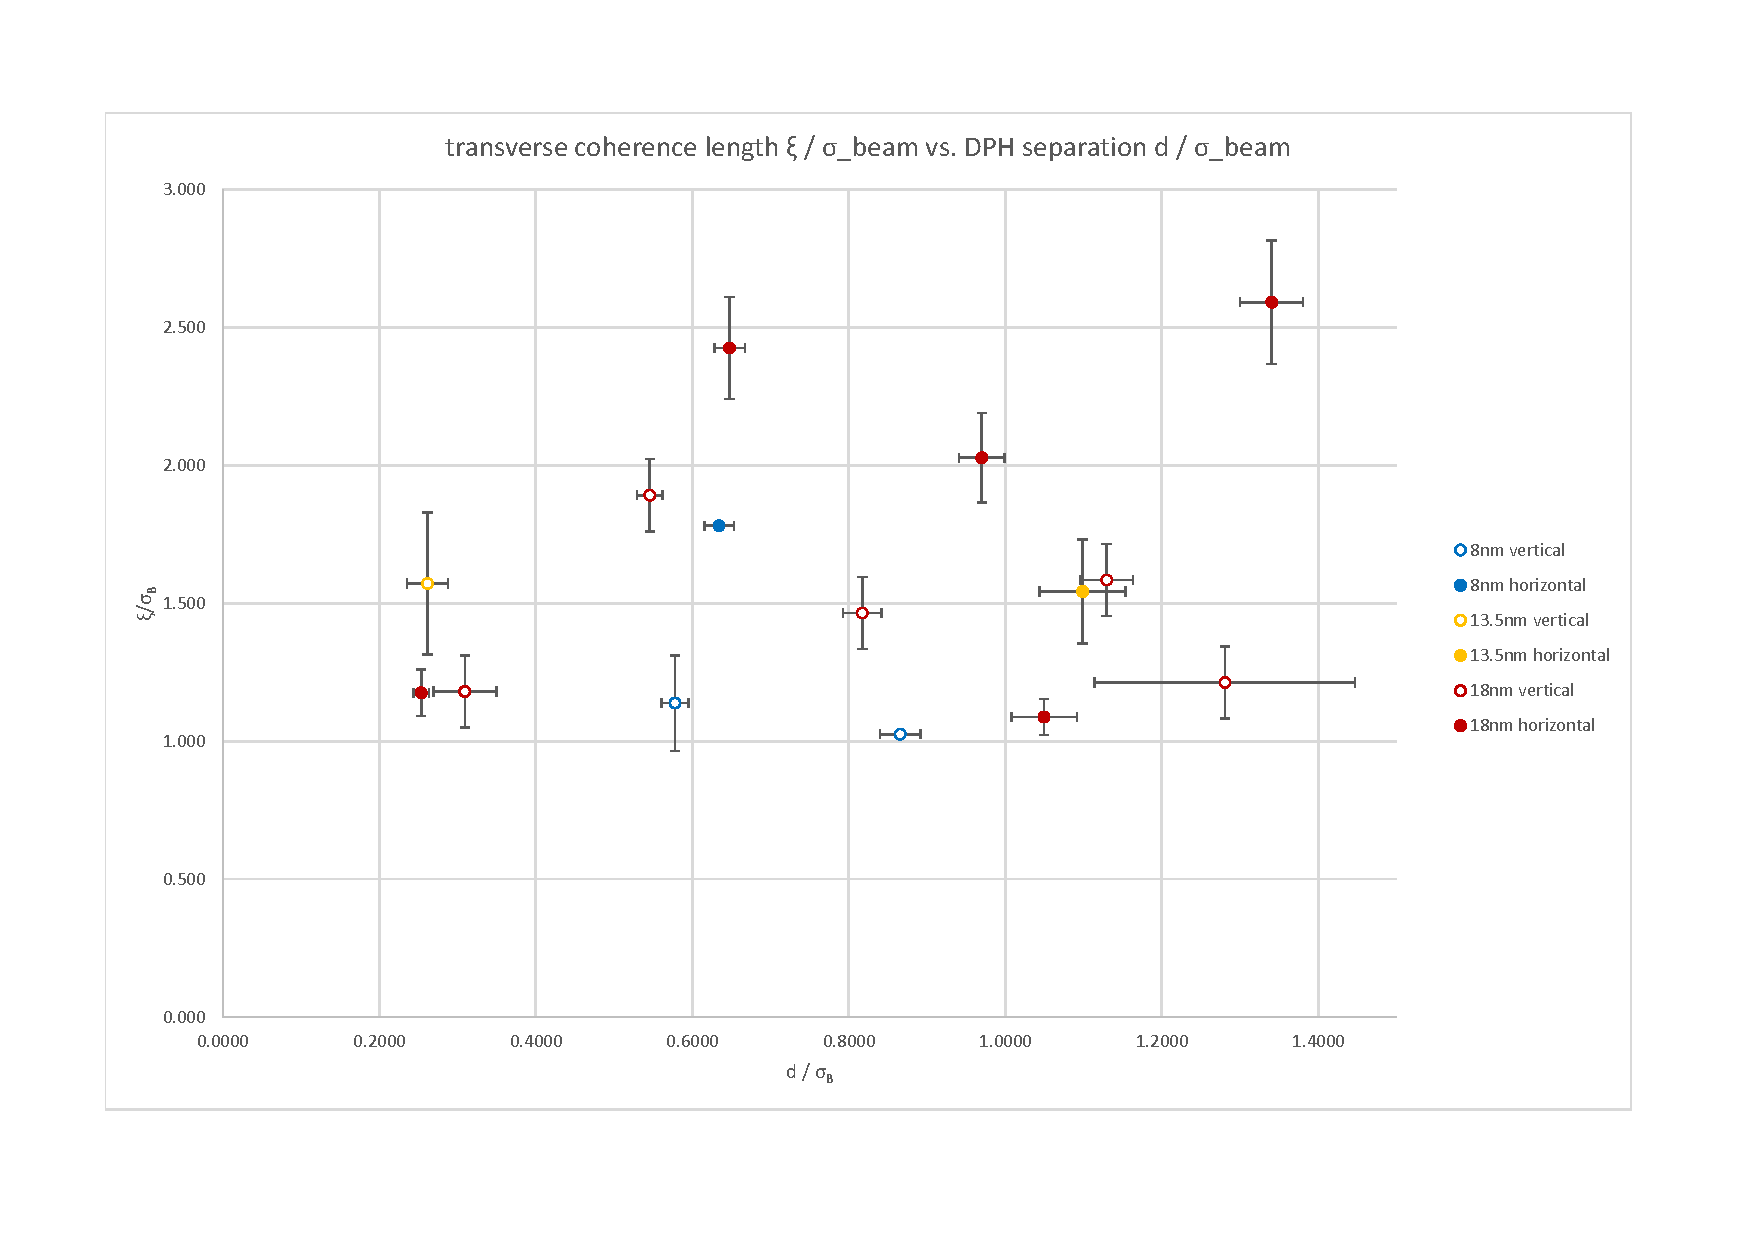
\includegraphics[width=1\textwidth]{gfx/xi_over_sigma_wiener_singelshot.pdf}
    \caption{Coherence length in relation to the pinhole separation determined from single-shot analysis using Wiener-deconvolution method.}
    \label{fig:DPH_results_coherence_vs_separation}
\end{figure}

\section{Future work}



%%%%%%%%%%%%%%%%%%%%%%% References %%%%%%%%%%%%%%%%%%%%%%%%%

%%%%%%%%%% If using BibTeX:
\bibliography{DP-Experiment}



\end{document}
